\documentclass[11pt,a4paper]{article}
\usepackage[utf8]{inputenc}
\usepackage[T1]{fontenc}
\usepackage[margin=0.88in]{geometry}
\usepackage{lmodern}
\usepackage{microtype}
\usepackage{amsmath,amssymb,mathtools}
\usepackage{graphicx}
\usepackage{booktabs,multirow,array}
\usepackage[section]{placeins}
\usepackage[numbers,sort&compress]{natbib}
\usepackage{xcolor}
\usepackage{enumitem}
\usepackage{hyperref}

\hypersetup{
    colorlinks=true,
    linkcolor=blue!50!black,
    citecolor=teal!55!black,
    urlcolor=blue!50!black,
    pdftitle={Uni-Loom: Predictor-Agnostic 3D Molecular Weaving with Dual-Track Valence Purity and Grounded Recursive Self-Improvement},
    pdfauthor={Shangqian Chen, Guojiang Zhao, Zheng Cheng, Jiankun Wang, Hongshuai Wang, Zhifeng Gao}
}

\setlength{\emergencystretch}{2em}
\widowpenalty=10000
\clubpenalty=10000
\displaywidowpenalty=10000
\setlength{\parskip}{0.32em}
\setlength{\parindent}{1.2em}
\setlength{\belowcaptionskip}{5pt}
\renewcommand{\topfraction}{0.90}
\renewcommand{\bottomfraction}{0.85}
\renewcommand{\textfraction}{0.08}
\renewcommand{\floatpagefraction}{0.82}

\title{\textbf{Uni-Loom: Predictor-Agnostic 3D Molecular Weaving with Dual-Track Valence Purity and Grounded Recursive Self-Improvement}}

\author{
Shangqian Chen, Guojiang Zhao, Zheng Cheng,\\
Jiankun Wang, Hongshuai Wang, Zhifeng Gao\\[4pt]
\small DP Technology, Beijing, China\\
\small\texttt{\{chensq, zhaogj, chengz, wangjk, wanghs, gaozf\}@dp.tech}
}

\date{November 2026}

\begin{document}
\maketitle

\begin{abstract}
Training a single monolithic 3D molecular generator from scratch to simultaneously master covalent valence grammar, equilibrium interatomic mechanics, synthetic accessibility, and calibrated multi-property control across diverse chemical regimes remains prohibitively expensive. Meanwhile, specialized foundation models for 3D autoregressive generation (\texttt{Uni-3DAR}), 3D/2D property prediction (\texttt{Uni-Mol}, \texttt{Uni-Mol2}, enterprise QSAR ensembles), and universal machine-learning interatomic potentials (\texttt{DPA-4}, \texttt{HyFF}) have matured independently. Here we introduce \textbf{Uni-Loom}, a four-layer predictor-agnostic weaving and grounded recursive self-improvement (RSI) framework that binds heterogeneous pretrained 3D generators, external property predictors, analytical chemistry rules, and interatomic potentials into a calibrated, anti-reward-hacking discovery loop without retraining external predictors. First, we resolve two structural pathologies of bondless 3D point-cloud generation---cross-scale policy-gradient interference and exotic zwitterionic artifacts (\texttt{[C-]}, \texttt{[O+]}, \texttt{[B-]}, halonium)---via scale-decoupled alignment (coarse-topology \texttt{TopoGRPO} paired with detached $0.01\,\text{\AA}$ sub-voxel equilibrium coordinate distillation) and a dual-track valence engine combining generation-side bond-order-aware neutral coordination guards with a zero-heavy-atom-RMSD \texttt{ValenceReconciler}. Second, we design a declarative \texttt{TaskWeavingSpec} and \texttt{CompositeCriticBus} supporting zero-retrain mounting of differentiable 3D predictors, black-box QSAR models, inequality constraints (e.g., $\text{SA\_Score} \le 3.5$, reactive \texttt{SMARTS}), and applicability-domain auditors. Third, we formulate a heteroscedastic dual-uncertainty atlas (\texttt{GPAtlas}) that orthogonally decomposes generative control spread $\sigma_{\text{gen}}(t)$ from epistemic calibration uncertainty $\sigma_{\text{cal}}(t)$, driving a four-quadrant \textbf{Grounded RSI} engine that freezes reinforcement learning in predictor blindspots while routing diverse scaffolds to external quantum-chemical calibration via a zero-retrain \texttt{ResidualCalibratedAsset}. Across strict scaffold-disjoint evaluations on \texttt{OE62} ($47{,}807$ 3D conformers; $1{,}792$ end-to-end proposals per benchmark), \textbf{Uni-Loom} lifts conditional calibration slope from $0.409$ to $1.00$, accelerates single-GPU decoding $7.29\times$ to $32.5\,\text{mol/s}$, raises 3D covalent legality to $98.5\%\text{--}99.3\%$ ($95.2\%\text{--}97.4\%$ on raw unedited point clouds), eliminates exotic zwitterions from $25.7\%$ to $0.00\%$ ($3.6\%\text{--}8.3\%$ raw) at exact $0.0000\,\text{\AA}$ heavy-atom RMSD, boosts synthesizable clean hits by $+66.1\%$ while shrinking cross-foundation surrogate hacking gaps $4.6\times$ ($0.655 \to 0.143\,\text{eV}$), and achieves a $4.40\times$ monotonic gain in blind-audited constrained clean hits ($52 \to 229 / 1{,}792$) over two Grounded RSI rounds while cutting blind deep-\texttt{HOMO} \texttt{DFT} error by $33.8\%$ with zero base-predictor weights modified. Finally, head-to-head \texttt{OE62} scaling against geometry-complete flow matching (\texttt{PropMolFlow} trained to $52.0\,\text{GPU-h}$ convergence), coarse-to-fine octree mid-tree pruning (\texttt{OctreeProcessCritic} $16\to 4$), size-anchored weaving (\texttt{[homo, n\_atoms]}), and $0.12\,\text{GPU-h}$ ($56$-step) hot-swapped online flow alignment (\texttt{Loom-AWR}) with dual-mode \texttt{PBE0/def2-TZVP} verification ($42$ prompts) demonstrate $17\times$ lower training compute and $2.6\text{--}2.9\times$ faster test-time throughput ($3.54\,\text{mol/s}$) for \textbf{Uni-Loom} alongside $75.2\%\text{--}76.0\%$ surrogate ($52.5\%\text{--}52.9\%$ blind) synthesizable yield and $0.270\,\text{eV}$ unbiased \texttt{PBE0} HOMO MAE ($54.8\%$ quantum hit yield) when weaving \texttt{PropMolFlow} via \texttt{Loom-AWR}.
\end{abstract}

\section{Introduction}
\label{sec:intro}

Inverse design of functional three-dimensional (3D) organic molecules---spanning optoelectronic semiconductors \citep{stuke2020oe62,bhat2023ocelot,zhao2026o2gen}, catalysts, and drug-like scaffolds \citep{hoogeboom2022edm,xu2023geoldm,zeng2026propmolflow}---requires satisfying a stringent conjunction of criteria: valid closed-shell Lewis bonding, low-strain 3D equilibrium geometry, synthetic accessibility \citep{ertl2009sa}, and precise targeting of continuous electronic or physicochemical properties. While recent equivariant diffusion \citep{hoogeboom2022edm,xu2023geoldm}, flow-matching \citep{zeng2026propmolflow}, and octree-based 3D autoregressive models \citep{lu2025uni3dar} have substantially improved unconditional 3D structure generation, deploying conditional 3D molecular generation as a reliable industrial platform faces three fundamental bottlenecks:

\begin{enumerate}[leftmargin=1.6em,itemsep=2pt,topsep=3pt]
    \item \textbf{Bondless Point-Cloud Valence Fragility and Surrogate Reward Hacking.} Modern 3D generators emit unbonded atomic point clouds $\mathcal{M} = \{(Z_i, \mathbf{r}_i)\}_{i=1}^N$ and rely on post-hoc distance-based bond perception such as \texttt{RDKit DetermineBonds} \citep{rdkit2026bonds}. Because hydrogen has a covalent radius of only $0.31\,\text{\AA}$, omitting or misplacing a single peripheral hydrogen across spatial octree boundaries---or placing a third neighbor near carbonyl/ether oxygen---forces neutral closed-shell bond perception ($\sum_i q_i = 0$) to assign high-energy zwitterionic formal charges such as \texttt{[C-]...[O+]}, \texttt{[B-]}, or halonium ions ($15\%\text{--}46\%$ of legal proposals in unaligned policies). Critically, we find on $4{,}737$ quantum-chemically evaluated generated conformers that large 3D property foundation models (\texttt{Uni-Mol2 1.1B} \citep{ji2024unimol2}) suffer severe out-of-distribution (OOD) error on such zwitterionic and strained geometries ($\text{MAE} = 0.720\,\text{eV}$ vs.\ \texttt{PBE0/def2-TZVP} \texttt{DFT}), turning online reinforcement learning (RL) into an adversarial exploit engine unless valence grammar and interatomic forces are internalized.
    \item \textbf{Siloed Predictor Assets and Task-Specific Coupling.} In practical pharmaceutical and materials pipelines, organizations already maintain mature, validated property predictors---including coordinate-differentiable 3D networks (\texttt{Uni-Mol} \citep{zhou2023unimol}), large 3D black-box ensembles (\texttt{Uni-Mol2} \citep{ji2024unimol2}), 2D fingerprint QSAR models, and analytical medicinal chemistry filters (\texttt{SA\_Score} \citep{ertl2009sa}, \texttt{QED} \citep{bickerton2012qed}, reactive \texttt{SMARTS}). Existing conditional 3D pipelines typically hard-code specific benchmark labels (e.g., \texttt{QM9} or \texttt{OE62} orbital energies) into bespoke training scripts or require joint retraining across targets that lack co-labeled training tables.
    \item \textbf{Blindspot-Induced Policy Collapse vs.\ Unguided Active Learning.} When a user requests targets near or beyond the support of historical training data, poor hit yield can stem from three distinct causes: (i) \emph{generator under-exploration} within a region where the predictor is trustworthy, (ii) \emph{predictor epistemic blindness} where the surrogate itself is uncalibrated, or (iii) \emph{chemical prior ceilings} where covalent organic density vanishes. Applying uniform RL across these regimes causes catastrophic reward hacking inside predictor blindspots, whereas naive active learning wastes expensive \texttt{DFT} or wet-lab budgets on strained or synthetically intractable molecules.
\end{enumerate}

To address these challenges cohesively, we present \textbf{Uni-Loom} (\texttt{loom v2.0}), a modular 3D molecular weaving architecture and grounded recursive self-improvement (RSI) platform (Figure~\ref{fig:architecture}). Rather than training a monolithic model from scratch, \textbf{Uni-Loom} weaves a pretrained 3D octree autoregressive generator (\texttt{Uni-3DAR} \citep{lu2025uni3dar}), plug-and-play external property assets, hot-swappable universal machine-learning interatomic potentials (\texttt{DPA-4} \citep{deepmodeling2026dpa4} and \texttt{HyFF} \citep{hyra2026hyff}), and an isolated cross-foundation audit oracle into a closed-loop system. Our main contributions are fourfold:

\begin{itemize}[leftmargin=1.5em,itemsep=2pt,topsep=3pt]
    \item \textbf{Predictor-Agnostic Three-Layer Weaving Bus:} We introduce a unified \texttt{PredictorAsset} protocol, declarative \texttt{TaskWeavingSpec}, and \texttt{CompositeCriticBus} that mount heterogeneous 3D differentiable predictors (exposing $\nabla_{\mathbf{R}}\hat{y}$ to a \texttt{PhysicsConstrainedCoordRefiner}), 3D/2D black-box QSAR models, and zero-conditioner-overhead inequality constraints (e.g., $\text{SA\_Score} \le 3.5$), backed by cross-oracle disagreement or single-oracle applicability-domain (\texttt{AD}) Tanimoto auditing.
    \item \textbf{Scale-Decoupled Alignment and Dual-Track Valence Purity:} We diagnose cross-scale gradient interference between coarse octree topology tokens and $0.01\,\text{\AA}$ sub-voxel coordinate tokens, decoupling coarse-topology policy optimization (\texttt{Stage 2.5A TopoGRPO}) from detached equilibrium coordinate distillation (\texttt{Stage 2.5B}, achieving $0.046\text{--}0.053\,\text{\AA}$ Kabsch relaxation RMSD). Paired with generation-side bond-order-aware neutral valence guards, an auxiliary \texttt{HeavyAtomValenceHead}, and a deterministic zero-heavy-RMSD \texttt{ValenceReconciler}, \textbf{Uni-Loom} achieves $95.2\%\text{--}97.4\%$ raw point-cloud legality and $98.5\%\text{--}99.3\%$ reconciled legality with $0.00\%$ exotic zwitterions.
    \item \textbf{Orthogonal Dual-Uncertainty \texttt{GPAtlas}:} We construct 1D and 2D heteroscedastic Gaussian-process atlases \citep{rasmussen2006gp} that separate generator spread $\sigma_{\text{gen}}(t)$ from empirical cross-foundation calibration uncertainty $\sigma_{\text{cal}}(t)$, exposing generative drift vector fields alongside narrow-gap OOD predictor divergence surfaces and providing a pre-generation gatekeeper for unreachable targets.
    \item \textbf{Grounded Recursive Self-Improvement (RSI) Engine:} Using a four-quadrant weak-zone state machine (\texttt{CONVERGED}, \texttt{INNER\_UNDEREXPLORED}, \texttt{OUTER\_BLINDSPOT}, \texttt{PRIOR\_CEILING}), \textbf{Uni-Loom} safely restricts zero-cost inner-loop RL to trusted intervals ($0\%$ RL weight on blindspots), exports Murcko-diverse \citep{bemis1996murcko} blindspot candidates for external \texttt{DFT} labeling, and updates a zero-retrain \texttt{ResidualCalibratedAsset} whose noise-subtracted epistemic variance causally unlocks blindspots for subsequent alignment rounds.
\end{itemize}

\begin{figure}[!t]
    \centering
    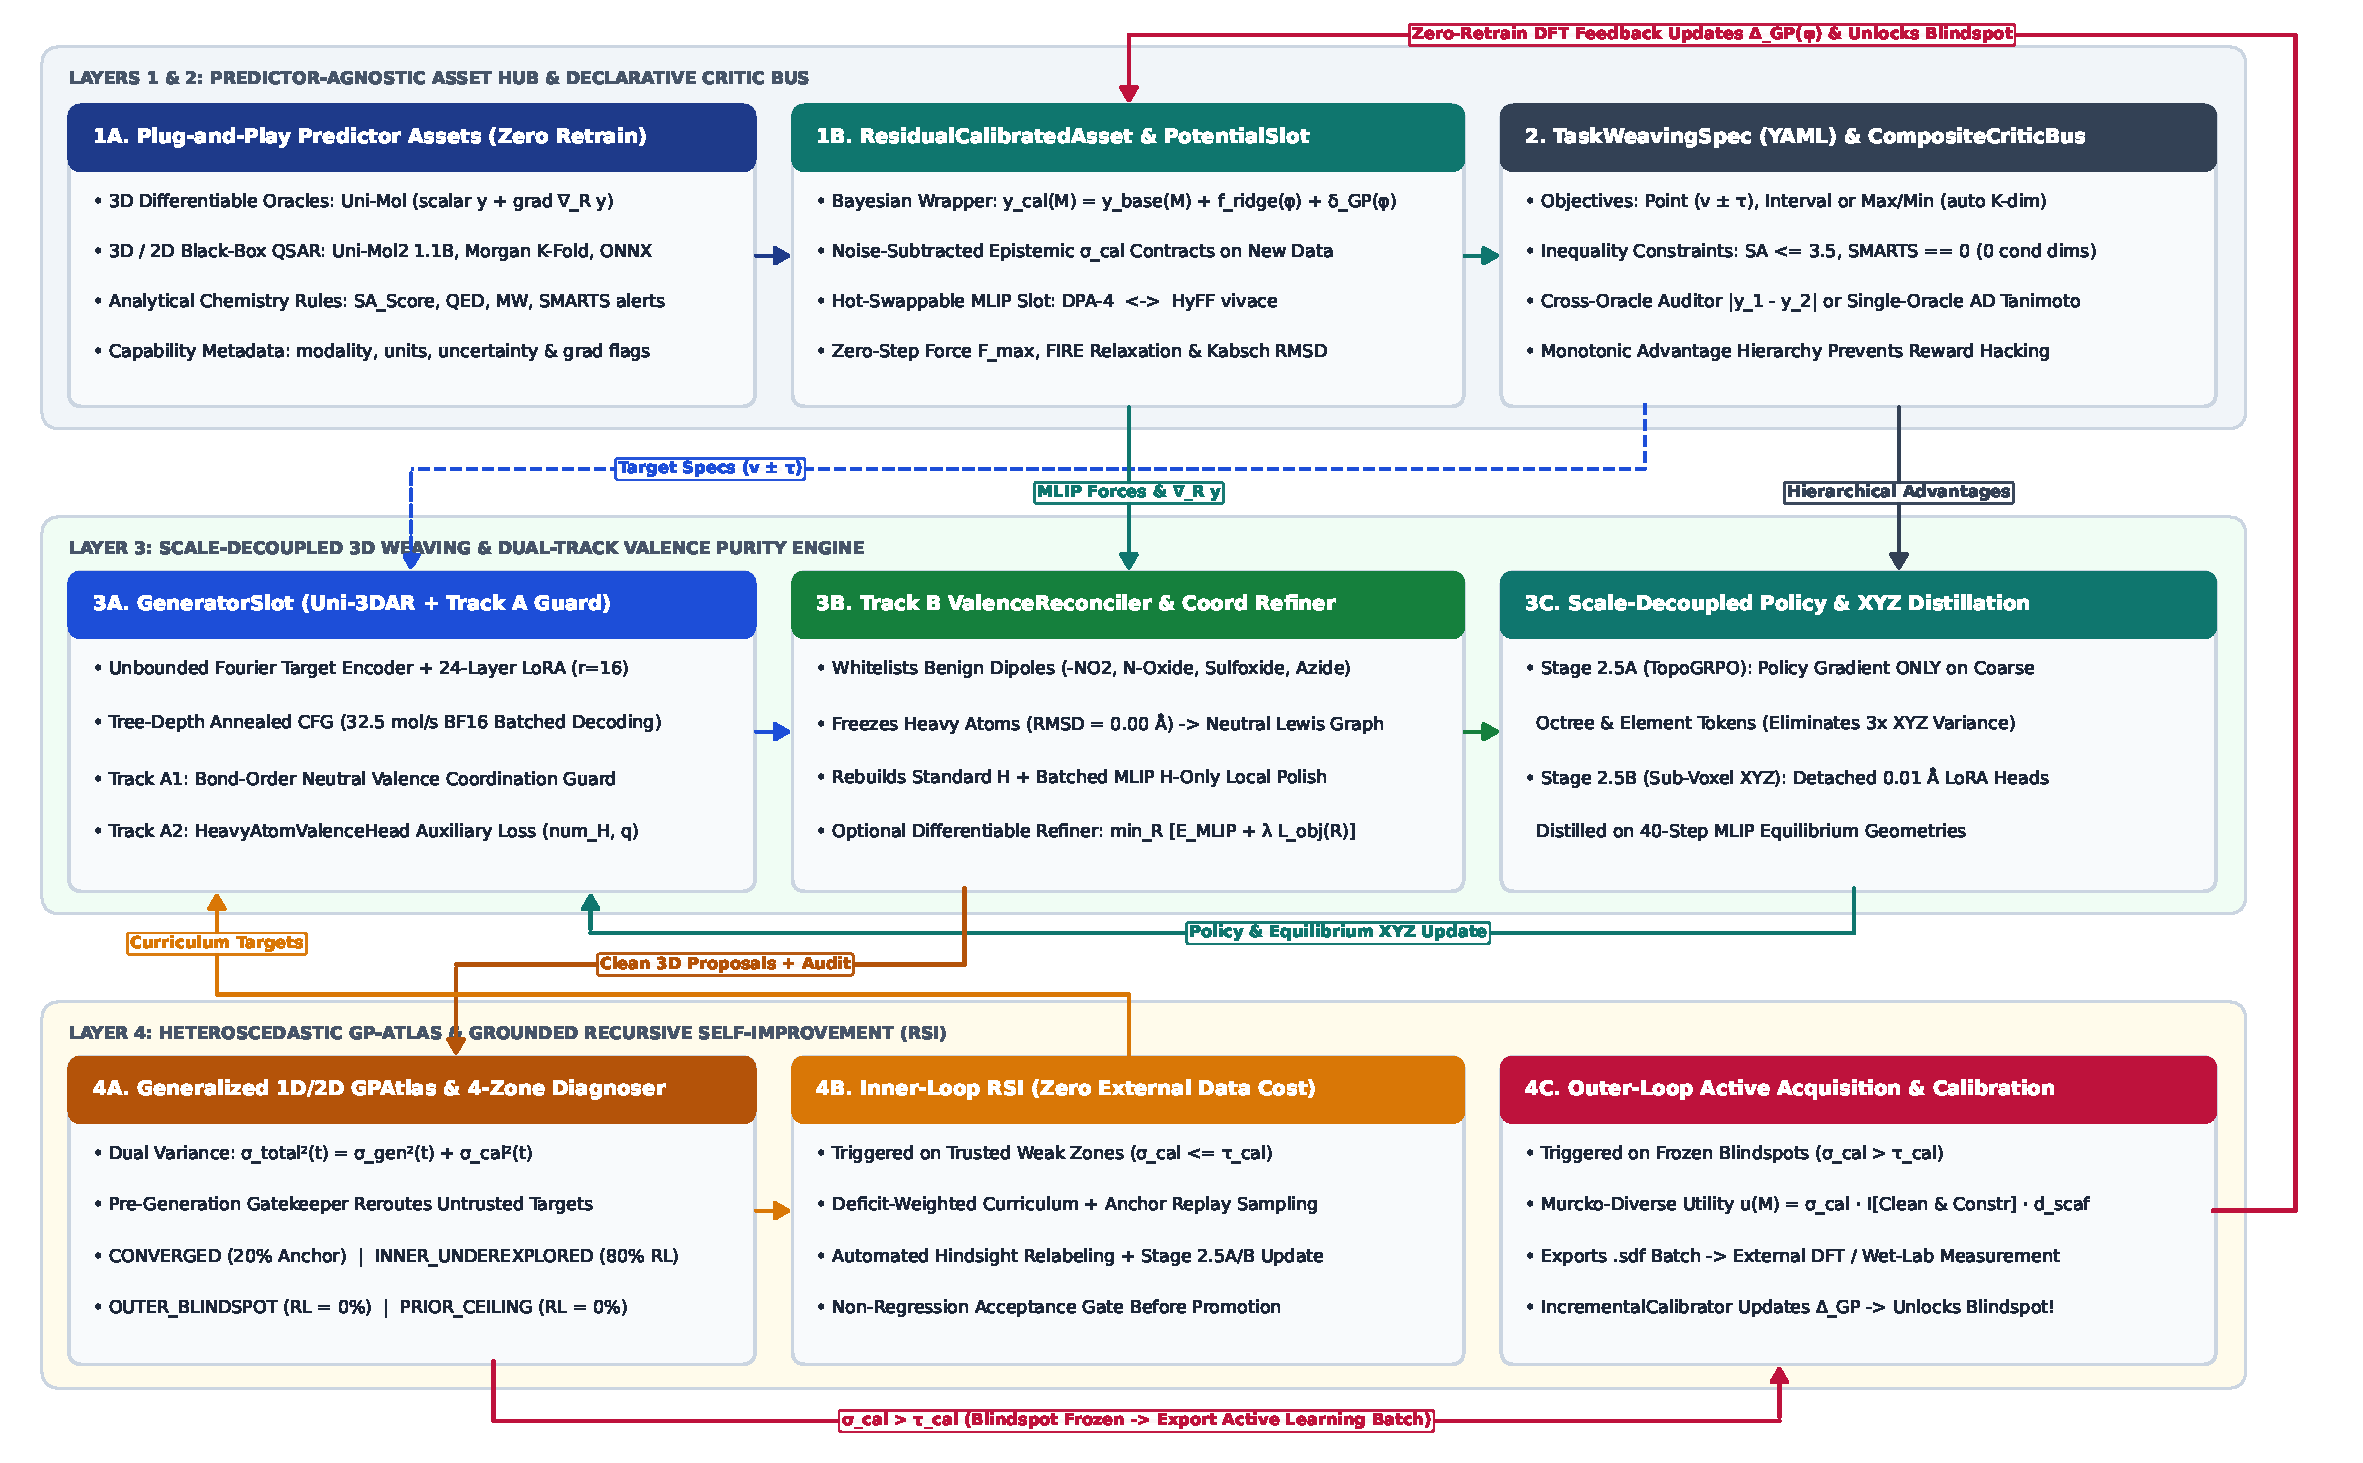
\includegraphics[width=\textwidth]{figures/fig1_uniloom_architecture.pdf}
    \caption{\textbf{Overview of the Uni-Loom (\texttt{loom v2.0}) weaving and grounded RSI architecture.} A five-stage forward pipeline connects declarative \texttt{TaskWeavingSpec} targets and inequality constraints (\texttt{SA\_Score}, \texttt{SMARTS}), octree autoregressive generation (\texttt{Uni-3DAR} with Track~A coordination guards and \texttt{HeavyAtomValenceHead}), zero-heavy-RMSD neutral graph reconciliation (Track~B \texttt{ValenceReconciler}), and a multi-asset \texttt{CompositeCriticBus} fed without retraining by the external asset hub (differentiable 3D models exposing $\nabla_{\mathbf{R}}\hat{y}$, black-box QSAR ensembles, \texttt{DPA-4}/\texttt{HyFF} potentials, and applicability-domain auditors). \texttt{GPAtlas} separates generative dispersion $\sigma_{\text{gen}}$ from calibration uncertainty $\sigma_{\text{cal}}$: trusted intervals ($\sigma_{\text{cal}} \le \tau_{\text{cal}}$) drive zero-external-cost scale-decoupled inner RSI (\texttt{Stage 2.5A TopoGRPO} on coarse tokens plus detached $0.01\,\text{\AA}$ sub-voxel distillation), whereas frozen blindspots ($\sigma_{\text{cal}} > \tau_{\text{cal}}$) route Murcko-diverse scaffolds to outer-loop \texttt{DFT} labeling and zero-retrain \texttt{ResidualCalibratedAsset} updates ($\Delta_{\text{GP}}$) while the blind \texttt{DPA-4} audit stays strictly isolated.}
    \label{fig:architecture}
\end{figure}

\section{Preliminaries and Problem Formulation}
\label{sec:prelim}

\subsection{Constrained Conditional 3D Molecular Generation}
Let $\mathcal{M} = (\mathbf{Z}, \mathbf{R}, \mathcal{G})$ denote a 3D molecular instance comprising $N$ atoms with atomic numbers $\mathbf{Z} \in \mathbb{Z}_+^N$, Cartesian coordinates $\mathbf{R} \in \mathbb{R}^{N \times 3}$, and an inferred closed-shell Lewis molecular graph $\mathcal{G} = (\mathcal{V}, \mathcal{E}, \mathbf{b}, \mathbf{q})$ with integer bond orders $\mathbf{b}$ and formal charges $\mathbf{q} \in \mathbb{Z}^N$ satisfying $\sum_{i=1}^N q_i = 0$. Given a vector of requested target specifications $\mathbf{t} = (t_1, \dots, t_K) \in \mathbb{R}^K$ with missingness mask $\mathbf{m} \in \{0,1\}^K$ and tolerances $\boldsymbol{\tau} = (\tau_1, \dots, \tau_K)$, together with $M$ auxiliary inequality constraints $\{g_j(\mathcal{M}) \le c_j\}_{j=1}^M$ (such as synthetic accessibility $\text{SA}(\mathcal{M}) \le 3.5$ or reactive-group count $\text{SMARTS}(\mathcal{M}) \le 0$), our goal is to learn a conditional generative policy $\pi_\theta(\mathcal{M} \mid \mathbf{t}, \mathbf{m})$ that maximizes the \emph{calibrated, constraint-satisfying, valence-clean hit yield}:
\begin{equation}
\label{eq:problem}
\begin{aligned}
\mathcal{Y}_{\text{clean}}(\mathbf{t}) = \mathbb{E}_{\mathcal{M} \sim \pi_\theta(\cdot \mid \mathbf{t}, \mathbf{m})} \!\Bigg[ \mathbb{I}\!\Bigg(
&\mathcal{M} \in \mathcal{V}_{\text{3D}} \;\land\; \mathcal{Q}_{\text{exotic}}(\mathcal{M}) = \emptyset \\
&\land\; \bigcap_{j=1}^M \{g_j(\mathcal{M}) \le c_j\} \;\land\; \bigcap_{k: m_k=1} \big\{|y_k^\star(\mathcal{M}) - t_k| \le \tau_k\big\}
\Bigg) \Bigg],
\end{aligned}
\end{equation}
where $\mathcal{V}_{\text{3D}}$ denotes single-component 3D covalent validity surviving interatomic potential relaxation without bond-graph rearrangement, $\mathcal{Q}_{\text{exotic}}(\mathcal{M})$ denotes unauthorized non-zero formal charges outside benign dipolar functional groups, and $y_k^\star(\mathcal{M})$ is the true quantum-chemical or experimental observable.

\subsection{Quantum Reference Consolidation and Surrogate Discrepancy Diagnosis}
\label{sec:quantum_audit}
A central premise of \textbf{Uni-Loom} is that a single surrogate oracle used to optimize $\pi_\theta$ cannot simultaneously serve as its own unbiased evaluator. To quantify surrogate vulnerability on generated 3D geometries, we consolidated historical \texttt{PBE0/def2-TZVP/DF} \texttt{DFT} single-point calculations \citep{sun2020pyscf,li2024gpu4pyscf,stuke2020oe62} across diverse generated and reference cohorts, strictly excluding all canonical molecular graphs and Murcko scaffolds overlapping held-out validation and test splits. This yielded $4{,}737$ leak-free generated 3D \texttt{DFT} structures ($3{,}949$ train, $398$ validation, $390$ test), which we merged with the scaffold-disjoint \texttt{OE62} training split ($43{,}858$ molecules) into a unified $47{,}807$-conformer pool (\texttt{oe62\_master\_train\_B}).

Evaluating two structurally distinct 3D foundation families on the $390$ held-out generated \texttt{DFT} test conformers reveals a striking fidelity gap: frozen \texttt{Uni-Mol2 1.1B} \citep{ji2024unimol2} (\texttt{RewardOracle}) exhibits test $\text{HOMO}/\text{LUMO}$ mean absolute errors (MAEs) of $0.720 / 0.778\,\text{eV}$ ($\text{RMSE} = 1.106 / 1.253\,\text{eV}$) due to sensitivity to subtle bond-length strain and formal-charge artifacts, whereas an independent \texttt{DFT}-calibrated \texttt{DPA-4} electronic head \citep{deepmodeling2026dpa4} (\texttt{AuditOracle}) achieves $0.186 / 0.183\,\text{eV}$ MAE ($\text{RMSE} = 0.268 / 0.268\,\text{eV}$). Throughout this work, \texttt{Uni-Mol2} (or a restricted historical QSAR ensemble in Section~\ref{sec:exp_rsi}) serves exclusively on the training side, while the calibrated \texttt{DPA-4} electronic head is strictly isolated as a blind \texttt{AuditOracle} that never participates in relabeling, filtering, or policy gradients.

\section{The Uni-Loom Architecture}
\label{sec:method}

\subsection{Layers 1 \& 2: Predictor-Agnostic Asset Hub and Declarative Critic Bus}
\label{sec:asset_bus}

\paragraph{Unified \texttt{PredictorAsset} Registry.}
To eliminate task-specific hard-coding and reuse mature industrial models without retraining, Layer~1 (\texttt{src/loom/weaving/registry.py}) wraps arbitrary property evaluators under a common \texttt{PredictorAsset} interface exposing machine-readable \texttt{AssetCapabilities} (\texttt{modality}, \texttt{is\_3d\_differentiable}, \texttt{has\_uncertainty}, \texttt{target\_names}, \texttt{units}). Four asset families mount out of the box:
\begin{enumerate}[leftmargin=1.6em,itemsep=1pt,topsep=2pt]
    \item \textbf{Differentiable 3D Deep Models (\texttt{UniMol3DAsset}):} Wraps coordinate-differentiable 3D backbones \citep{zhou2023unimol} to provide both batched scalar predictions $\hat{\mathbf{y}}(\mathcal{M})$ and analytical Cartesian gradients $\nabla_{\mathbf{R}}\hat{y}_k(\mathbf{Z}, \mathbf{R})$ via autograd on pairwise distance encodings;
    \item \textbf{Black-Box 3D \& 2D QSAR Assets (\texttt{SlotOracleAsset}, \texttt{FingerprintQSARAsset}, \texttt{CallablePredictorAsset}):} Wraps frozen 3D foundation models (\texttt{Uni-Mol2}), $K$-fold Morgan fingerprint ensembles (returning epistemic ensemble standard deviation $\sigma_{\text{ens}}$), or external \texttt{ONNX}/\texttt{scikit-learn} callables;
    \item \textbf{Zero-Cost Analytical Chemistry Rules (\texttt{BuiltInRuleAsset}):} Computes exact topological and medicinal descriptors including \texttt{SA\_Score} \citep{ertl2009sa}, \texttt{QED} \citep{bickerton2012qed}, molecular weight, rotatable-bond count, maximum ring size, strained $3/4$-membered ring counts, and reactive/unstable functional-group \texttt{SMARTS} alerts (peroxides, acyl halides, nitroso, strained heterocycles);
    \item \textbf{Hot-Swappable Interatomic Potentials (\texttt{PotentialSlot}):} Unifies \texttt{DPA-4} \citep{deepmodeling2026dpa4} and \texttt{HyFF vivace} \citep{hyra2026hyff} behind precision-safe \texttt{float64} spatially separated batch packing (reducing batch-$32$ packing force numerical drift from $7.09 \times 10^{-3}$ to $7.89 \times 10^{-6}\,\text{eV/\AA}$), providing zero-step maximum atomic force $F_{\max}$, batched \texttt{FIRE} relaxation, graph-preservation checks, and Kabsch-aligned relaxation deformation $\text{RMSD}_{\text{Kabsch}}$ (with graceful \texttt{NaN} fallback on unsupported heavy elements such as $\text{Te}$).
\end{enumerate}

\paragraph{Physics-Constrained Differentiable Coordinate Refinement.}
When a mounted objective asset exposes \texttt{is\_3d\_differentiable=True}, \texttt{PhysicsConstrainedCoordRefiner} jointly optimizes conformer coordinates on the composite potential surface:
\begin{equation}
\label{eq:coord_refine}
\min_{\mathbf{R} \in \mathbb{R}^{N \times 3}} \; E_{\text{MLIP}}(\mathbf{Z}, \mathbf{R}) + \lambda \sum_{k=1}^K w_k \, \mathcal{L}_{\text{obj}, k}\!\big(\hat{y}_k(\mathbf{Z}, \mathbf{R}); t_k, \tau_k\big),
\end{equation}
where clipped interatomic forces $-\nabla_{\mathbf{R}} E_{\text{MLIP}}$ lock covalent bond lengths and angles inside physical equilibrium basins while $-\lambda \nabla_{\mathbf{R}}\mathcal{L}_{\text{obj}, k}$ steers soft torsional degrees of freedom toward the target window, guarded by a strict graph-preservation and maximum-force acceptance check relative to both initial and current coordinates.

\paragraph{Declarative \texttt{TaskWeavingSpec} and Monotonic \texttt{CompositeCriticBus}.}
Layer~2 (\texttt{spec.py}, \texttt{critic\_bus.py}) compiles declarative YAML specifications into three orthogonal channels:
(i) \textbf{Objectives} (\texttt{point}, \texttt{interval}, \texttt{max}, or \texttt{min}), which automatically configure the generator's conditioning dimension $K$ and impute missing multi-model pseudo-labels across unlabeled 3D conformer pools;
(ii) \textbf{Inequality Constraints} ($g_j(\mathcal{M}) \le c_j$ with soft margin $s_j$ and hard-gate flag), which shape feasibility without consuming conditioning dimensions; and
(iii) \textbf{Anti-Hacking Auditors}. Crucially, when a second foundation oracle is unavailable---the norm in proprietary industrial QSAR deployments---the bus automatically activates \texttt{single\_oracle\_ad} mode, combining nearest-neighbor Morgan fingerprint Tanimoto applicability-domain distance $d_{\text{AD}}(\mathcal{M}) = 1 - \max_{\mathcal{M}' \in \mathcal{D}_{\text{ref}}} \text{Sim}(\mathcal{M}, \mathcal{M}')$, ensemble standard deviation $\sigma_{\text{ens}}(\mathcal{M})$, target-range extrapolation penalties, and 3D potential strain gates. Across online rollouts, \texttt{CompositeCriticBus} enforces a strict monotonic reward hierarchy:
\begin{equation}
\label{eq:hierarchy}
R_{\text{clean+constr+hit}} > R_{\text{clean+constr+miss}} > R_{\text{soft-constr-viol}} > R_{\text{exotic-charge / high-strain}} > R_{\text{illegal-3D}},
\end{equation}
ensuring that no property-surrogate outlier can ever outscore a valence-clean, low-strain, constraint-satisfying molecule.

\subsection{Layer 3: Scale-Decoupled 3D Weaving}
\label{sec:scale_decoupled}

\paragraph{Removing Conditioning Bottlenecks and Accelerating Octree Decoding.}
We bind \texttt{Uni-3DAR} \citep{lu2025uni3dar} as \texttt{GeneratorSlot} (\texttt{LoomUni3DARGenerator}). Inspection of early adapter baselines revealed that per-layer adaptive LayerNorm modulation had been hard-clipped by $0.08 \tanh(\cdot)$ with frozen attention layers, capping conditional calibration slope at $0.41\text{--}0.54$. We remove the $\tanh$ bottleneck, inject continuous Fourier features of $(\mathbf{t}, \mathbf{m})$ alongside rank-$16$ \texttt{LoRA} adapters \citep{hu2022lora} across all $24$ Transformer blocks, train with paired conditional/unconditional dropout ($p_{\text{drop}} = 0.15$) plus a contrastive conditioning auxiliary loss, and apply tree-depth annealed classifier-free guidance (\texttt{CFG} \citep{ho2022cfg}) at inference:
\begin{equation}
\label{eq:cfg}
\ell_{\text{CFG}}(u \mid d) = \ell_{\text{uncond}}(u) + \Big(1 + (s_{\text{CFG}} - 1)\,\gamma^{\max(d - d_0, 0)}\Big)\big(\ell_{\text{cond}}(u) - \ell_{\text{uncond}}(u)\big),
\end{equation}
which concentrates strong target steering at coarse scaffold-determining octree levels ($d \le d_0$) while annealing guidance at fine leaf levels to preserve local bond geometry. Vectorized dual-branch \texttt{BF16} batching with fused scaled dot-product attention increases single-\texttt{A800} generation throughput from $4.46\,\text{mol/s}$ to $32.52\,\text{mol/s}$ ($7.29\times$ speedup at batch $256$, and $22.3\text{--}29.5\,\text{mol/s}$ with dual-pass \texttt{CFG} and GPU geometric guards enabled).

\paragraph{Why Coarse Topology RL and Sub-Voxel Coordinate Distillation Must Be Decoupled.}
In octree autoregressive decoding, each leaf atom emits \emph{four} tokens across disparate length scales: one coarse chemical-identity token ($Z_i$, sampled at $T_Z = 0.30$) and three $0.01\,\text{\AA}$ sub-voxel coordinate offset tokens ($\Delta x_i, \Delta y_i, \Delta z_i$, sampled at $T_{xyz} = 0.25$). Propagating a molecule-level scalar electronic reward advantage $A_{\text{prop}}$ through all tokens (\emph{coupled RL}) injects $3\times$ token-count credit-assignment variance into shared Transformer representations: empirically (Section~\ref{sec:exp_progression}), coupled RL + online relaxation distillation achieves excellent local mechanics ($\text{RMSD}_{\text{Kabsch}} = 0.049\,\text{\AA}$, legality $88.6\%$) but degrades within-target property spread $\sigma_{\text{in}}$ from $0.439$ to $0.534\,\text{eV}$.

\textbf{Uni-Loom} resolves this conflict by decoupling the two spatial scales:
\begin{enumerate}[leftmargin=1.6em,itemsep=2pt,topsep=2pt]
    \item \textbf{Stage 2.5A (\texttt{TopoGRPO}):} Group-relative policy optimization \citep{shao2024grpo} ($G = 8\text{--}16$ proposals per target prompt) restricts the policy-gradient mask exclusively to coarse octree-subdivision and element-type tokens ($\mathcal{T}_{\text{topo}}$), zeroing policy gradients on fine \texttt{XYZ} tokens and computing exact dual-finite token-level KL divergence against the reference policy (eliminating all \texttt{NaN} KL instabilities induced by hard logit masks):
    \begin{equation}
    \label{eq:topogrpo}
    \begin{aligned}
    \mathcal{L}_{\text{TopoGRPO}}(\theta) = -\mathbb{E}_{g, i}\!\Bigg[\frac{1}{|\mathcal{T}_{\text{topo}}^{(i)}|} \sum_{u \in \mathcal{T}_{\text{topo}}^{(i)}} \Big( &\min\!\big(\rho_u A_i, \text{clip}(\rho_u, 1-\epsilon, 1+\epsilon)A_i\big) \\
    &-\; \beta_{\text{KL}} D_{\text{KL}}^{\text{finite}}(\pi_\theta \| \pi_{\text{ref}})_u \Big)\Bigg] + \lambda_{\text{rep}} \mathcal{L}_{\text{SFT}}^{\text{replay}}.
    \end{aligned}
    \end{equation}
    \item \textbf{Stage 2.5B (Detached Sub-Voxel Equilibrium Distillation):} Freezing the conditioner, 24-layer Transformer, and topology/element heads via \texttt{hidden.detach()}, we attach lightweight rank-$8$ \texttt{LoRA} adapters ($111{,}744$ parameters) solely to the three $0.01\,\text{\AA}$ \texttt{XYZ} heads and supervise them on $40$-step \texttt{MLIP}-relaxed graph-preserving equilibrium conformers, compressing zero-step atomic strain without perturbing coarse property calibration.
\end{enumerate}

\paragraph{Mid-Tree Process Weaving (\texttt{Octree\allowbreak Process\allowbreak Critic}) and Hot-Swappable \texttt{Generator\allowbreak Slot}.}
Because fine leaf-atom and $0.01\,\text{\AA}$ coordinate decoding consume $65\%\text{--}80\%$ of octree generation wall-clock time, \textbf{Uni-Loom} introduces \texttt{Octree\allowbreak Process\allowbreak Critic} (\texttt{octree\_\allowbreak process\_\allowbreak critic.py}) right at the coarse-to-fine octree boundary ($\text{level } 1 \to 0$). Pooling conditioned 24-layer KV-cached prefix representations (\texttt{h\_root}, \texttt{h\_coarse\_mean}, \texttt{h\_l1\_mean}, \texttt{h\_l1\_last}) alongside $14$ $\text{SO}(3)$-invariant coarse voxel envelope descriptors (leaf-slot counts $K_1, K_2$, bounding spans, radius of gyration, inertial eigenvalues $\lambda_{1..3}$, planarity, and tree log-perplexity), the critic predicts conditional property mean/variance $(\hat{\mu}_{\text{proc}}, \log\sigma_{\text{proc}}^2)$, 3D legality $\ell_{\text{legal}}$, and constraint feasibility $\ell_{\text{constr}}$, pruning $M_{\text{init}} \to M_{\text{keep}}$ KV-cached branches (e.g., $16 \to 4$, or $8 \to 1$ with zero external surrogate calls) prior to leaf decoding. Furthermore, \texttt{Generator\allowbreak Slot} is strictly paradigm-agnostic: alongside discrete autoregressive \texttt{Loom\allowbreak Uni3DAR\allowbreak Generator}, \texttt{Loom\allowbreak FlowMol\allowbreak Generator} (\texttt{flowmol\_\allowbreak slot.py}) mounts continuous-time Markov chain (CTMC) + $\text{SE}(3)$ flow-matching models (\texttt{PropMolFlow} \citep{zeng2026propmolflow}) behind the identical critic bus and supports online Advantage-Weighted Regression (\texttt{Loom-AWR}, \texttt{awr\_sft}), weighting clean rollouts by $\exp(A_i / \beta_{\text{AWR}})$ combining strict native-legality gating, online $20$-step \texttt{MLIP} coordinate relaxation with post-relaxation critic re-verification, and curated $\text{SA}\le 3.5$ equilibrium conformer replay.

\subsection{Dual-Track Elimination of Exotic Zwitterions}
\label{sec:valence}

\paragraph{Root-Cause Analysis.}
Why do unaligned 3D point-cloud policies produce $15\%\text{--}26\%$ exotic formal charges (\texttt{[C-]}, \texttt{[O+]}, \texttt{[B-]}, halonium) despite trained exclusively on neutral closed-shell molecules? In \texttt{Uni-3DAR}, heavy-atom skeletons are often geometrically sound, but (i) an oxygen atom placed within $< 1.65\,\text{\AA}$ of three heavy/H neighbors becomes trivalent oxonium \texttt{[O+]}, or (ii) missing one peripheral hydrogen on an $sp^3$/$sp^2$ carbon while placing an extra hydrogen near a carbonyl oxygen forces \texttt{DetermineBonds(..., charge=0)} \citep{rdkit2026bonds} to pair \texttt{[C-]} with \texttt{[O+]} to conserve total neutrality and even electron count. We eliminate this artifact via two synergistic tracks (always reporting \emph{Raw Point-Cloud} and \emph{Valence-Reconciled} metrics side by side):

\begin{itemize}[leftmargin=1.5em,itemsep=2pt,topsep=2pt]
    \item \textbf{Track A (Generation-Side Suppression in \texttt{uni3dar\_slot.py}):} During GPU batched octree decoding, we enforce a \emph{Bond-Order-Aware Neutral Valence Coordination Guard} directly on pre-softmax element logits \citep{lu2025uni3dar}: if an existing oxygen already has one short double-bond neighbor ($d < 1.28\,\text{\AA}$, e.g., $\text{C=O}$) or two covalent neighbors, any new atom falling within covalent bonding distance of that oxygen has its bonding logits masked before \texttt{softmax}; halogens ($\text{F, Cl, Br, I}$) lock immediately at coordination $1$, and boron ($\text{B}$) locks at neutral trivalent coordination $3$, blocking oxonium, halonium, and \texttt{[B-]} formation at sampling time. Simultaneously, we mount a lightweight linear \texttt{HeavyAtomValenceHead} ($< 30\text{K}$ parameters) on \texttt{atom\_heads[0]} hidden states during SFT and replay to predict each heavy atom's canonical attached hydrogen count $n_{\text{H}} \in \{0,\dots,4\}$ and formal charge state $q \in \{-1, 0, +1\}$, forcing the trunk representation to internalize local valence conservation.
    \item \textbf{Track B (Zero-Heavy-RMSD \texttt{ValenceReconciler} in \texttt{valence\_reconciler.py}):} At point-cloud reconstruction, we inspect formal charges against a strict whitelist of benign neutral dipolar motifs (nitro \texttt{[N+](=O)[O-]}, $N$-oxide, sulfoxide, and diazo/azide). Any raw point cloud that is already covalently valid and clean is returned \emph{completely untouched} (\texttt{clean\_raw}). Only when an unauthorized zwitterion or isolated peripheral-H count mismatch occurs on an intact, collision-free, single-component heavy-atom skeleton, \texttt{ValenceReconciler} freezes all heavy-atom 3D coordinates ($\text{RMSD}_{\text{heavy}} \equiv 0.0000\,\text{\AA}$), infers a neutral closed-shell integer Lewis bond-order assignment from 3D interatomic distances and bond angles, rebuilds ideal-geometry explicit hydrogens, and executes $10$ batched H-only \texttt{MLIP} relaxation steps with frozen heavy atoms before re-verifying connectivity and closed-shell sanitization.
\end{itemize}

\subsection{Layer 4: Heteroscedastic \texttt{GPAtlas} and Grounded RSI Engine}
\label{sec:rsi}

\paragraph{Orthogonal Dual-Uncertainty Decomposition (\texttt{GPAtlas}).}
Given a target grid $\mathcal{T} \subset \mathbb{R}^D$ ($D \in \{1, 2\}$), \texttt{HeteroscedasticGPAtlas} fits three smooth Gaussian-process surfaces over empirical proposal cohorts: (i) achieved conditional mean $\hat{\mu}_{\text{gen}}(\mathbf{t})$, (ii) intrinsic generator dispersion $\sigma_{\text{gen}}(\mathbf{t})$, and (iii) epistemic calibration uncertainty $\sigma_{\text{cal}}(\mathbf{t})$ (measured via cross-foundation disagreement RMSE when an audit oracle is available, or via \texttt{ResidualCalibratedAsset} posterior uncertainty / applicability-domain proxy in single-oracle mode), alongside empirical evaluability probability $p_{\text{eval}}(\mathbf{t})$. The calibrated probability of achieving a true hit within window $[t_k - \tau_k, t_k + \tau_k]$ integrates over total orthogonal variance $\sigma_{\text{total}}^2(\mathbf{t}) = \sigma_{\text{gen}}^2(\mathbf{t}) + \sigma_{\text{cal}}^2(\mathbf{t})$:
\begin{equation}
\label{eq:phit}
P_{\text{hit}}^{\text{cal}}(\mathbf{t}) = p_{\text{eval}}(\mathbf{t}) \prod_{k=1}^D \left[ \Phi\!\left(\frac{t_k + \tau_k - \hat{\mu}_{\text{gen}, k}(\mathbf{t})}{\sqrt{\sigma_{\text{gen}, k}^2(\mathbf{t}) + \sigma_{\text{cal}, k}^2(\mathbf{t})}}\right) - \Phi\!\left(\frac{t_k - \tau_k - \hat{\mu}_{\text{gen}, k}(\mathbf{t})}{\sqrt{\sigma_{\text{gen}, k}^2(\mathbf{t}) + \sigma_{\text{cal}, k}^2(\mathbf{t})}}\right) \right].
\end{equation}
Mounted at inference as a \emph{Pre-Generation Gatekeeper} (\texttt{recommend\_target}), \texttt{GPAtlas} intercepts queries where $P_{\text{hit}}^{\text{cal}}(\mathbf{t})$ or $\sigma_{\text{cal}}(\mathbf{t})$ violates trust thresholds and recommends the nearest reachable Pareto target.

\paragraph{Four-Quadrant Diagnostic State Machine and Dual-Loop Flywheel.}
At each RSI round, \texttt{RSIDiagnoser} classifies every target cell $\mathbf{t} \in \mathcal{T}$ into four actionable causal states:
\begin{enumerate}[leftmargin=1.6em,itemsep=2pt,topsep=2pt]
    \item \textbf{\texttt{PRIOR\_CEILING}:} Vanishing source KDE density $\rho_{\text{src}}(\mathbf{t}) < \rho_{\min}$ accompanied by severe prior pull $|\hat{\mu}_{\text{gen}}(\mathbf{t}) - \mathbf{t}| > \tau_{\text{ceil}}$ $\implies$ \emph{curriculum RL weight set to $0\%$}, flagging need for novel chemical element/scaffold priors;
    \item \textbf{\texttt{OUTER\_BLINDSPOT}:} Calibration uncertainty exceeds trust cap $\sigma_{\text{cal}}(\mathbf{t}) > \tau_{\text{cal}}$ $\implies$ \emph{inner-loop RL weight frozen at $0\%$} to prevent surrogate reward hacking, triggering \texttt{OuterRSIAcquisition} to rank clean, low-strain, constraint-satisfying candidates by Murcko-scaffold-diversified \citep{bemis1996murcko} utility:
    \begin{equation}
    \label{eq:acq}
    u(\mathcal{M}) = \sigma_{\text{cal}}(\mathcal{M}) \cdot \mathbb{I}\big[\text{Clean}(\mathcal{M}) \land \text{ConstraintsMet}(\mathcal{M})\big] \cdot d_{\text{Murcko}}(\mathcal{M}, \mathcal{S}_{\text{selected}}),
    \end{equation}
    exporting \texttt{acquisition\_batch.sdf} for high-precision \texttt{DFT} or experimental measurement;
    \item \textbf{\texttt{INNER\_UNDEREXPLORED}:} Predictor is trusted ($\sigma_{\text{cal}}(\mathbf{t}) \le \tau_{\text{cal}}$) but $P_{\text{hit}}^{\text{cal}}(\mathbf{t}) < p_{\text{conv}}$ $\implies$ receives $80\%$ of adaptive curriculum probability weighted by hit-deficit $(1 - P_{\text{hit}}^{\text{cal}}(\mathbf{t}))$ for zero-external-cost \texttt{InnerRSIRunner} (\texttt{Hindsight} relabeling + \texttt{Stage 2.5A/B}), guarded by a non-regression acceptance gate;
    \item \textbf{\texttt{CONVERGED}:} Trusted ($\sigma_{\text{cal}}(\mathbf{t}) \le \tau_{\text{cal}}$) and $P_{\text{hit}}^{\text{cal}}(\mathbf{t}) \ge p_{\text{conv}}$ $\implies$ retains $20\%$ anchor replay budget to mitigate catastrophic forgetting.
\end{enumerate}

\paragraph{Zero-Retrain Bayesian Residual Calibration (\texttt{ResidualCalibratedAsset}).}
When external ground-truth labels $\{(\mathcal{M}_i, y_i^{\text{true}})\}_{i=1}^{N_{\text{fb}}}$ return from the outer loop while the external base predictor $\hat{y}_{\text{base}}$ remains a frozen black box, \texttt{IncrementalCalibrator} maps each molecule to a compact $20$-dimensional normalized descriptor $\boldsymbol{\phi}(\mathcal{M}) \in \mathbb{R}^{20}$ ($16$-channel folded Morgan bit-density fingerprint plus molecular weight, heavy-atom fraction, aromatic-carbon fraction, and heteroatom ratio) and fits a global \texttt{Ridge} bias-trend estimator $f_{\text{ridge}}(\boldsymbol{\phi})$ plus a fixed-prior-amplitude $\text{Mat\'ern}(\nu=3/2) + \text{WhiteKernel}$ Gaussian process $\delta_{\text{GP}}(\boldsymbol{\phi})$ on the detrended residuals $r_i = y_i^{\text{true}} - \hat{y}_{\text{base}}(\mathcal{M}_i) - f_{\text{ridge}}(\boldsymbol{\phi}_i)$:
\begin{equation}
\label{eq:rescal}
\begin{aligned}
\hat{y}_{\text{cal}}(\mathcal{M}) &= \hat{y}_{\text{base}}(\mathcal{M}) + f_{\text{ridge}}\!\big(\boldsymbol{\phi}(\mathcal{M})\big) + \delta_{\text{GP}}\!\big(\boldsymbol{\phi}(\mathcal{M})\big), \\
\sigma_{\text{epistemic}}(\mathcal{M}) &= \sqrt{\max\!\Big(\sigma_{\text{GP}}^2\big(\boldsymbol{\phi}(\mathcal{M})\big) - \sigma_{\text{noise}}^2,\, 0\Big)}.
\end{aligned}
\end{equation}
Separating the global OOD bias shift $f_{\text{ridge}}$ from the fixed-prior local GP kernel and subtracting estimated observation noise $\sigma_{\text{noise}}^2$ guarantees that ingesting authentic \texttt{DFT} anchors monotonically contracts $\sigma_{\text{cal}}(\mathbf{t})$ below $\tau_{\text{cal}}$, causally transitioning \texttt{OUTER\_BLINDSPOT} intervals into \texttt{INNER\_UNDEREXPLORED}/\texttt{CONVERGED} for the next inner-loop alignment round without modifying a single weight of $\hat{y}_{\text{base}}$.

\section{Experimental Validation}
\label{sec:experiments}

\subsection{Experimental Setup, Benchmarks, and Throughput Scaling}
\label{sec:exp_setup}

All primary benchmarks are conducted on the scaffold-disjoint \texttt{OE62} crystal-forming organic semiconductor dataset \citep{stuke2020oe62} augmented with our leak-free consolidated quantum pool ($47{,}807$ training conformers up to $80$ atoms spanning $11$ elements: $\text{H, B, C, N, O, F, Si, P, S, Cl, Br, I}$). Every end-to-end conditional evaluation uses the identical held-out protocol and deterministic random streams (\texttt{seeds [24411, 24412]}): $7$ quantile targets ($P_{10}, P_{25}, P_{35}, P_{50}, P_{65}, P_{75}, P_{90}$) $\times$ $256$ proposals $= 1{,}792$ uncurated end-to-end proposals per evaluation, with hit tolerance $\tau = \pm 0.25\,\text{eV}$. Following strict denominator transparency, failed or non-evaluable proposals are never discarded from hit-yield denominators.

Table~\ref{tab:speed} summarizes single-\texttt{NVIDIA A800-80GB} decoding and training throughput. Replacing legacy \texttt{FP32} per-row stream loops with vectorized \texttt{BF16} octree decoding and fused attention delivers $32.52\,\text{mol/s}$ at batch $256$ ($5.07\times$ over matched batch-$32$ \texttt{FP32} and $7.29\times$ over the legacy $4.46\,\text{mol/s}$ pipeline) while consuming only $3.23\,\text{GB}$ peak VRAM; training throughput increases to $80.92\,\text{mol/s}$ even with $2\times$-pass contrastive conditioning enabled.

\begin{table}[!t]
\centering
\caption{Single-\texttt{NVIDIA A800-80GB} generation and training throughput scaling (\texttt{speed\_benchmark.json}, $256$ molecules per sampling arm).}
\label{tab:speed}
\resizebox{\textwidth}{!}{%
\begin{tabular}{llrrrr}
\toprule
Pipeline Configuration & Precision & Batch & CFG Scale & Peak VRAM (GB) & Throughput (mol/s) \\
\midrule
Legacy baseline pipeline (per-row \texttt{FP32} loop) & \texttt{FP32} & 32 & 1.00 & --- & 4.46 \\
Vectorized \texttt{FP32} row-streams baseline & \texttt{FP32} & 32 & 1.00 & --- & 6.41 \\
\textbf{Uni-Loom} (\texttt{BF16} fused octree decoding) & \texttt{BF16} & 64 & 1.00 & 1.92 & 11.75 \\
\textbf{Uni-Loom} (\texttt{BF16} fused octree decoding) & \texttt{BF16} & 128 & 1.00 & 2.39 & 20.19 \\
\textbf{Uni-Loom} (\texttt{BF16} fused octree decoding) & \texttt{BF16} & 256 & 1.00 & 3.23 & \textbf{32.52} ($7.29\times$) \\
\textbf{Uni-Loom} (dual-branch \texttt{CFG} + geometric guard) & \texttt{BF16} & 128--256 & 1.75--2.00 & 3.36 & \textbf{22.25--29.51} \\
\midrule
Training: Legacy \texttt{FP32} SFT (single pass, no contrast) & \texttt{FP32} & 32 & --- & --- & 72.85 \\
Training: \textbf{Uni-Loom} \texttt{BF16} \texttt{LoRA-16} + $2\times$ contrastive pass & \texttt{BF16} & 32 & --- & --- & \textbf{80.92} ($1.11\times$) \\
\bottomrule
\end{tabular}%
}
\end{table}

\subsection{End-to-End Stage Progression, Anti-Reward-Hacking Audit, and Potential Hot-Swap}
\label{sec:exp_progression}

Table~\ref{tab:progression} and Figure~\ref{fig:progression} track end-to-end \texttt{OE62 HOMO} generation across legacy baselines and \textbf{Uni-Loom} Stages $0 \to 2.5$ ($1{,}792$ proposals). Removing the $0.08\tanh$ conditioning bottleneck in Stage~0 immediately lifts calibration slope from $0.409$ to $0.934$ and compresses within-target spread $\sigma_{\text{in}}$ from $0.570$ to $0.420\,\text{eV}$, yet raw zero-step legality is only $59.6\%$ with $60.8\%$ exotic charges and blind \texttt{AuditOracle} MAE of $1.536\,\text{eV}$. Incorporating \texttt{DPA-4} graph-preserving Hindsight relabeling (Stage~1) and monotonic disentangled \texttt{GRPO} (Stage~2) raises end-to-end hit yield to $34.60\%$ ($620/1{,}792$) while slashing post-relaxation blind \texttt{AuditOracle} MAE from $1.536$ to $0.757\,\text{eV}$.

\begin{table}[!t]
\centering
\caption{End-to-end \texttt{OE62 HOMO} conditional generation progression across $1{,}792$ proposals ($7$ quantiles $\times 256$, tolerance $\pm 0.25\,\text{eV}$, raw unedited point-cloud evaluation prior to \texttt{v2.0} reconciliation). \texttt{Audit MAE} is evaluated by the strictly isolated \texttt{DFT}-calibrated \texttt{DPA-4} electronic oracle.}
\label{tab:progression}
\resizebox{\textwidth}{!}{%
\begin{tabular}{lrrrrrrrr}
\toprule
Method / Stage & Hits / 1792 & Hit Yield & Clean Hits & 3D Legal & Slope & $\sigma_{\text{in}}$ (eV) & Reward MAE & Blind Audit MAE \\
\midrule
Legacy Frozen SFT & 371 & 20.70\% & --- & 72.1\% & 0.409 & 0.570 & 0.521 & --- \\
Legacy Margin + \texttt{GRPO-1024} & 441 & 24.61\% & --- & 70.0\% & 0.535 & 0.542 & 0.451 & --- \\
\textbf{Uni-Loom} Stage 0 (\texttt{LoRA-16} + \texttt{CFG=1.75}) & 470 & 26.23\% & 184 (10.3\%) & 59.6\% & 0.934 & 0.420 & 0.347 & 1.536 \\
\textbf{Uni-Loom} Stage 1 (\texttt{DPA-4} Hindsight) & 528 & 29.46\% & 286 (16.0\%) & 63.6\% & 0.933 & \textbf{0.418} & \textbf{0.339} & 1.137 \\
\textbf{Uni-Loom v1.0} Stage 2 (\texttt{GRPO-1024}, \texttt{CFG=2.0}) & 620 & 34.60\% & 449 (25.1\%) & 80.5\% & 1.045 & 0.439 & 0.364 & 0.757 \\
\textbf{Uni-Loom v1.1} \texttt{GRPO-1024} + Guard + \texttt{XYZ} Distill & 625 & 34.88\% & 450 (25.1\%) & 80.1\% & 1.037 & 0.427 & 0.353 & 0.825 \\
\textbf{Uni-Loom v1.1} Stage 2.5A (\texttt{Guard+TopoGRPO}, \texttt{CFG=1.75}) & 604 & 33.71\% & 436 (24.3\%) & 84.6\% & \textbf{0.986} & 0.480 & 0.403 & \textbf{0.744} \\
\textbf{Uni-Loom v1.1} Stage 2.5A (\texttt{Guard+TopoGRPO}, \texttt{CFG=2.0}) & \textbf{631} & \textbf{35.21\%} & \textbf{451 (25.2\%)} & 83.5\% & 1.100 & 0.471 & 0.393 & 0.755 \\
\textbf{Uni-Loom v1.1} Stage 2.5A+2.5B (\texttt{TopoGRPO+XYZ}, \texttt{CFG=1.75}) & 615 & 34.32\% & 447 (24.9\%) & \textbf{85.4\%} & 0.985 & 0.475 & 0.400 & 0.903 \\
\bottomrule
\end{tabular}%
}
\end{table}

\begin{figure}[!t]
    \centering
    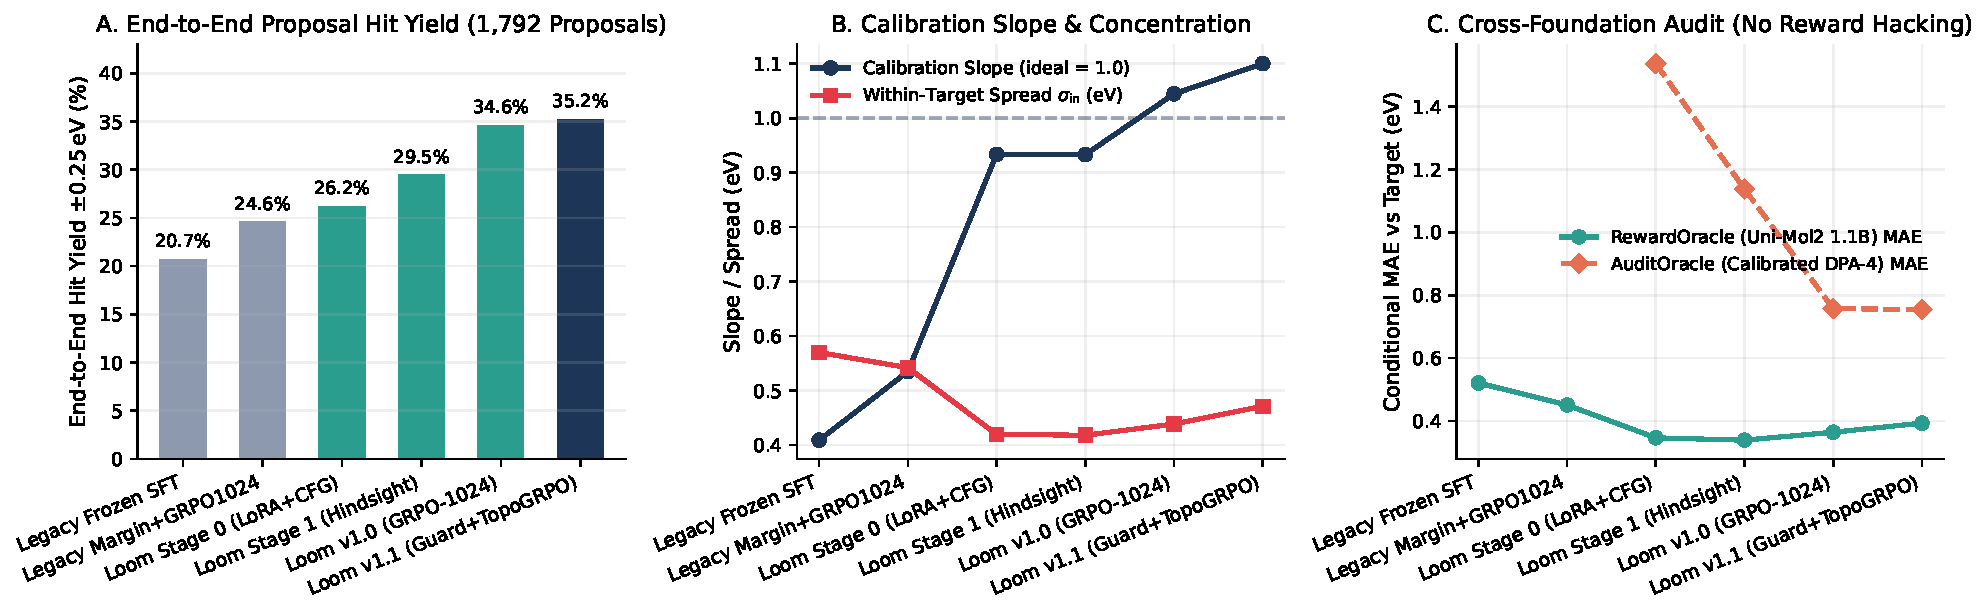
\includegraphics[width=\textwidth]{figures/fig2_stage_progression.pdf}
    \caption{\textbf{End-to-end \texttt{OE62 HOMO} progression across stages ($1{,}792$ proposals).} (\textbf{A}) End-to-end hit yield within $\pm 0.25\,\text{eV}$ rises $+70.1\%$ relative to Legacy Frozen SFT ($20.7\% \to 35.2\%$, $621$ novel unique molecular graphs). (\textbf{B}) Removing per-layer $\tanh$ clipping restores unit calibration slope ($\approx 1.0$) while tightening within-target spread $\sigma_{\text{in}}$. (\textbf{C}) Strictly isolated cross-foundation \texttt{AuditOracle} (\texttt{DFT}-calibrated \texttt{DPA-4}) MAE drops monotonically alongside \texttt{RewardOracle} alignment ($1.536 \to 0.755\,\text{eV}$), confirming genuine physical improvement rather than surrogate exploitation.}
    \label{fig:progression}
\end{figure}

\begin{figure}[!t]
    \centering
    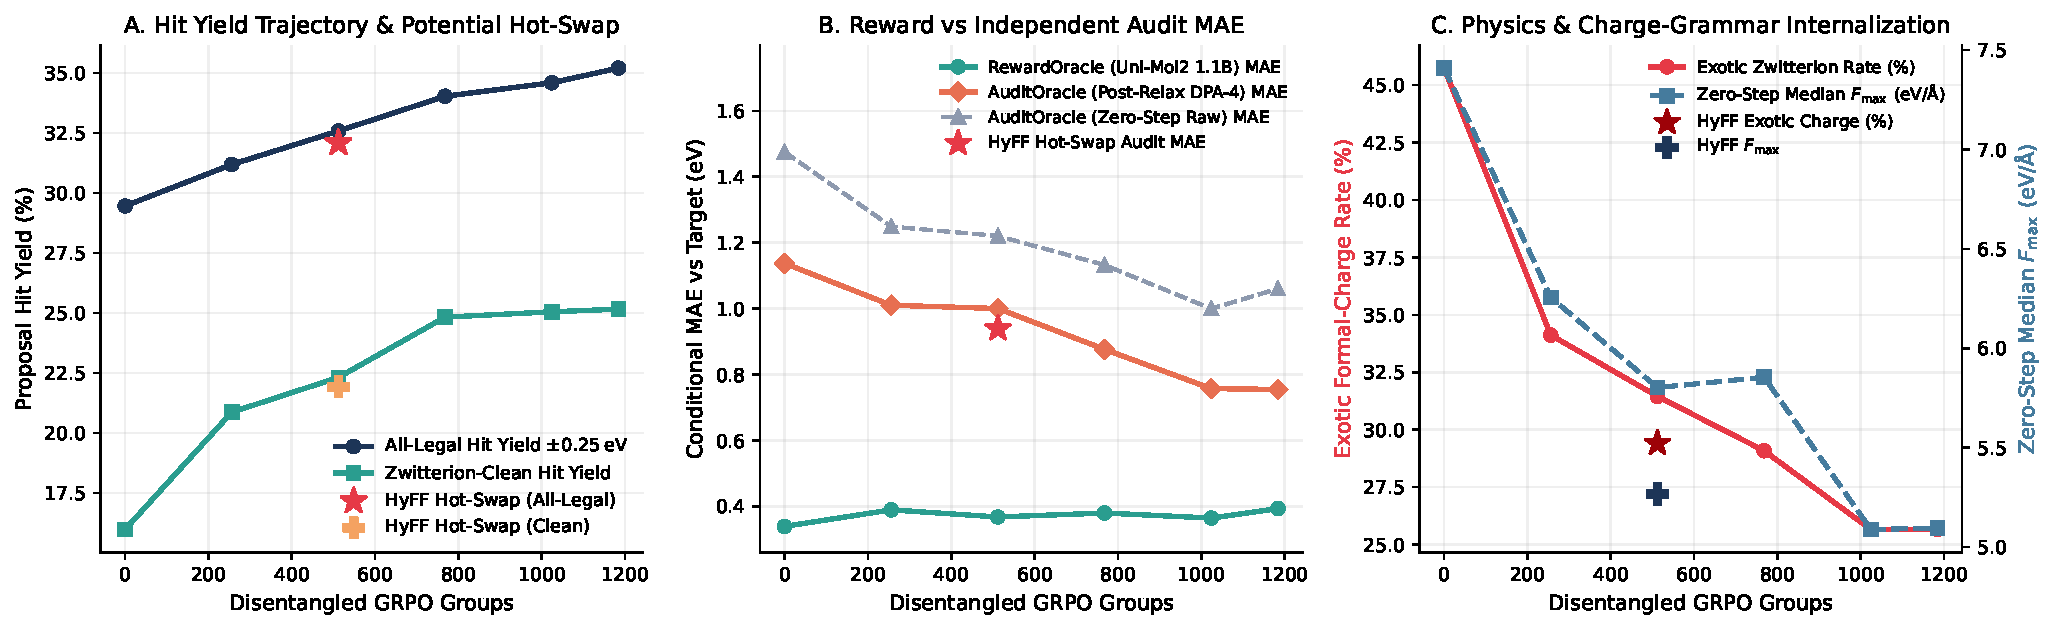
\includegraphics[width=\textwidth]{figures/fig3_audit_and_hotswap.pdf}
    \caption{\textbf{Online RL anti-reward-hacking trajectory ($0 \to 1{,}184$ groups) and zero-code \texttt{PotentialSlot} hot-swap.} (\textbf{A}) Total and zwitterion-clean hit yields rise monotonically with \texttt{GRPO} budget. (\textbf{B}) Independent post-relaxation \texttt{AuditOracle} MAE decreases steadily from $1.137$ to $0.755\,\text{eV}$ while \texttt{RewardOracle} MAE remains stable ($\approx 0.36\text{--}0.39\,\text{eV}$). (\textbf{C}) Exotic formal-charge rate and zero-step median $F_{\max}$ ($7.41 \to 5.09\,\text{eV/\AA}$) drop concurrently. Switching \texttt{PotentialSlot} at $512$ groups from \texttt{DPA-4} to \texttt{HyFF vivace} with zero code changes achieves lower zero-step forces ($5.27$ vs.\ $5.80\,\text{eV/\AA}$), higher graph-preserving relaxation ($88.3\%$ vs.\ $81.6\%$), and superior blind \texttt{Audit} MAE ($0.939$ vs.\ $1.000\,\text{eV}$).}
    \label{fig:audit_hotswap}
\end{figure}

\paragraph{Anti-Reward-Hacking Curve, Potential Hot-Swapping, and Scale-Decoupling Ablation.}
Figure~\ref{fig:audit_hotswap} evaluates checkpoints every $256$ \texttt{GRPO} groups from $0$ to $1{,}184$ groups. Rather than diverging---the classic signature of Goodhart's law---blind \texttt{AuditOracle} MAE drops monotonically ($1.137 \to 1.010 \to 1.000 \to 0.876 \to 0.757 \to 0.755\,\text{eV}$) as zero-step median force $F_{\max}$ falls from $7.41$ to $5.09\,\text{eV/\AA}$ and graph-preserving relaxation rises from $75.8\%$ to $90.6\%$. Hot-swapping \texttt{PotentialSlot} from \texttt{DPA-4} to \texttt{HyFF vivace} \citep{hyra2026hyff} at $512$ groups via a single CLI flag achieves $32.09\%$ hit yield ($575/1{,}792$) with lower $F_{\max}$ ($5.27\,\text{eV/\AA}$) and lower blind \texttt{Audit} MAE ($0.939\,\text{eV}$).

Table~\ref{tab:v11_ablation} isolates the effect of spatial scale decoupling (Section~\ref{sec:scale_decoupled}). Coupled online training (propagating scalar electronic rewards into $3\times$ sub-voxel \texttt{XYZ} tokens alongside online relaxation distillation) achieves remarkable mechanical equilibrium ($\text{RMSD}_{\text{Kabsch}} = 0.0495\,\text{\AA}$, $88.62\%$ legality, $F_{\max} = 4.19\,\text{eV/\AA}$) but inflates within-target electronic dispersion $\sigma_{\text{in}}$ to $0.534\,\text{eV}$, lowering hit count to $526$. By contrast, \texttt{Stage 2.5A TopoGRPO} restricts policy gradients to coarse topology/element tokens to achieve peak hit count ($631/1{,}792$, $621$ novel unique hit graphs, $0.744\,\text{eV}$ blind \texttt{Audit} MAE at \texttt{CFG=1.75}), while detached \texttt{Stage 2.5B} sub-voxel distillation compresses $\text{RMSD}_{\text{Kabsch}}$ to $0.0533\text{--}0.0579\,\text{\AA}$ and boosts raw legality to $85.38\%$.

\begin{table}[!t]
\centering
\caption{Ablation of spatial scale decoupling vs.\ coupled coordinate RL on \texttt{OE62 HOMO} ($1{,}792$ proposals, raw unedited point clouds). $\text{RMSD}_{\text{Kabsch}}$ measures heavy-and-H intrinsic conformational shift after $20$-step \texttt{DPA-4} relaxation.}
\label{tab:v11_ablation}
\resizebox{\textwidth}{!}{%
\begin{tabular}{lrrrrrrr}
\toprule
Ablation Arm & Hits (Clean) & 3D Legal & Exotic $Q$ & $\sigma_{\text{in}}$ (eV) & Median $F_{\max}$ (eV/\AA) & $\text{RMSD}_{\text{Kabsch}}$ (\AA) & Post-Relax Audit MAE \\
\midrule
\texttt{v1.0} Baseline (no guard, frozen \texttt{XYZ}) & 620 (449) & 80.47\% & 25.7\% & 0.439 & 5.09 & 0.0613 & 0.757 \\
$+$ Zero-shot 3D geometric guard + tree \texttt{CFG} & 622 (444) & 81.75\% & 25.5\% & 0.436 & 5.12 & 0.0586 & 0.811 \\
$+$ Detached $0.01\,\text{\AA}$ \texttt{XYZ} equilibrium distillation & 625 (450) & 81.81\% & 25.8\% & \textbf{0.427} & 5.19 & 0.0581 & 0.825 \\
\textbf{Stage 2.5A} (\texttt{Guard + TopoGRPO}, coarse tokens only) & \textbf{631 (451)} & 84.60\% & 25.3\% & 0.471 & 5.10 & 0.0559 & \textbf{0.744} \\
\textbf{Stage 2.5A + 2.5B} (cascaded decoupled) & 615 (447) & 85.38\% & 26.1\% & 0.475 & 5.18 & 0.0533 & 0.903 \\
Control: \emph{Coupled RL} (\texttt{XYZ} in policy + online distill) & 526 (402) & \textbf{88.62\%} & \textbf{17.2\%} & 0.534 & \textbf{4.19} & \textbf{0.0495} & 0.786 \\
\bottomrule
\end{tabular}%
}
\end{table}

\subsection{Joint Multi-Property Generation and Orthogonal 1D/2D \texttt{GPAtlas}}
\label{sec:exp_atlas}

Conditioning a single unified generator on $[\text{HOMO}, \text{LUMO}]$ simultaneously with missingness masks supports marginal and joint orbital design within one checkpoint. On marginal \texttt{LUMO} generation ($1{,}792$ proposals), upgrading from \texttt{v1.0} to \texttt{v1.1} ($40$-step \texttt{DPA-4} equilibrium pool + 3D geometric guard) elevates 3D covalent legality by $+12.0\,\text{pp}$ ($75.3\% \to 87.33\%$), cuts raw exotic charges from $27.1\%$ to $16.2\%$, reduces zero-step $F_{\max}$ by $25\%$ ($5.04 \to 3.79\,\text{eV/\AA}$), achieves $94.1\%$ graph-preserving relaxation with $\text{RMSD}_{\text{Kabsch}} = 0.0469\,\text{\AA}$, and reaches unit calibration slope ($1.002$ at \texttt{CFG=2.0}).

Figures~\ref{fig:atlas1d} and~\ref{fig:atlas2d} illustrate the 1D and 2D heteroscedastic \texttt{GPAtlas} built over $1{,}764$ relaxed, clean 3D proposals across a $7 \times 7$ $(\text{HOMO}, \text{LUMO})$ grid audited by the blind \texttt{DPA-4} oracle. In 1D (Figure~\ref{fig:atlas1d}), \texttt{GPAtlas} separates the reachability calibration geometry (Panel~A) from the hit-viability and prior-support profile (Panel~B): Panel~A uses equal-scale square coordinates ($[-9.5, -4.5]\,\text{eV}$ on both axes) to show posterior conditional mean $\hat{\mu}_{\text{gen}}(t)$ hugging the diagonal $y = t$ across $[-8.85, -5.77]\,\text{eV}$ before saturating above $-5.77\,\text{eV}$, while Panel~B plots surrogate vs.\ calibrated hit probabilities on an independent axis comparing the amber-shaded trusted reachable interval against the indigo source prior density curve. In 2D (Figure~\ref{fig:atlas2d}), replacing constant calibration heuristics with empirical cross-foundation disagreement yields two genuinely orthogonal diagnostic maps: Panel~A reveals clean joint hit yield peaking at $22.0\%$ alongside the generative drift vector field $\hat{\boldsymbol{\mu}}(\mathbf{t}) - \mathbf{t}$ pulling extreme queries toward the high-density organic semiconductor manifold, whereas Panel~B exposes a pronounced spatial gradient in cross-foundation uncertainty $\sigma_{\text{cal,2D}}$---ranging from $0.83\,\text{eV}$ in data-rich wide-gap regions ($t_{\text{H}} \in [-8.0, -7.0], t_{\text{L}} \in [-0.8, +0.2]\,\text{eV}$) to $1.14\,\text{eV}$ in narrow-gap push--pull donor--acceptor regimes ($t_{\text{H}} \in [-6.3, -5.7], t_{\text{L}} \in [-2.7, -1.5]\,\text{eV}$), pinpointing exactly where surrogate predictions require \texttt{DFT} verification.

\begin{figure}[!t]
    \centering
    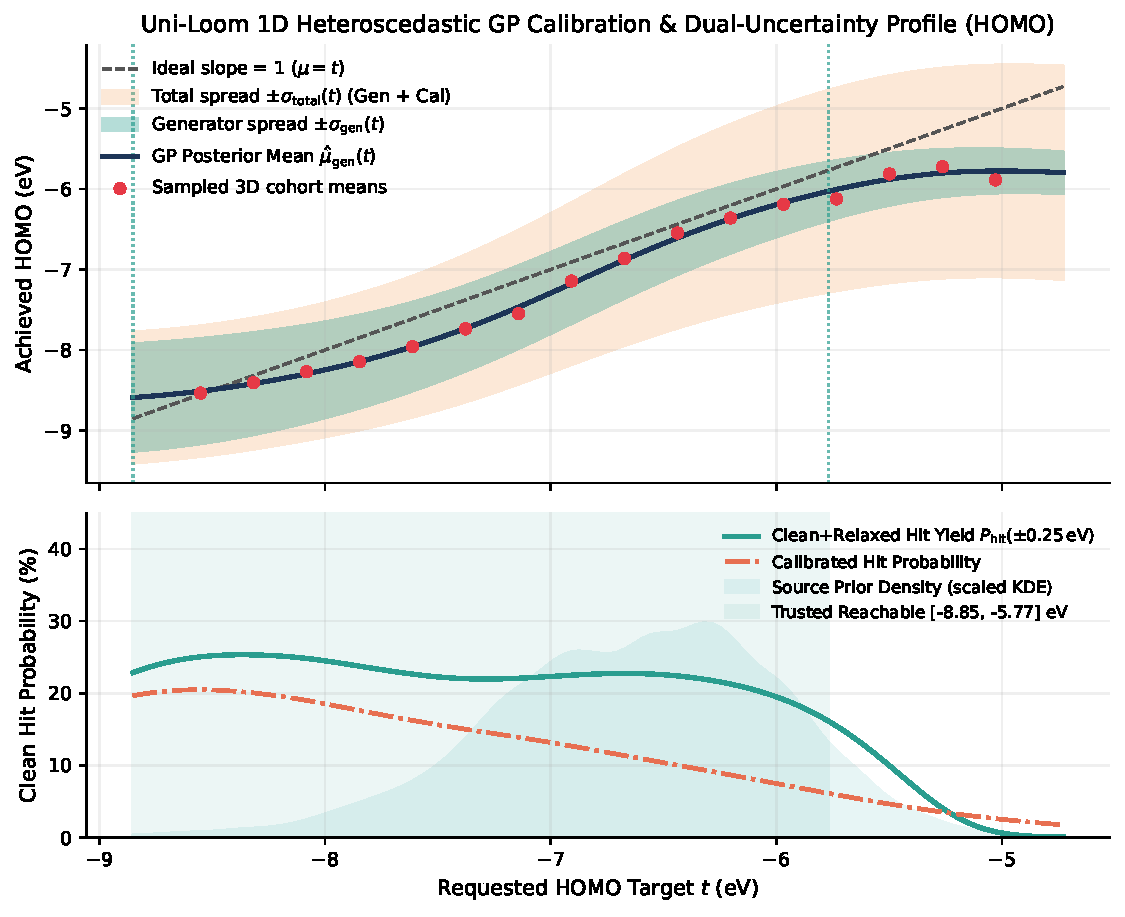
\includegraphics[width=\textwidth]{figures/fig4_gp_atlas_1d_homo.pdf}
    \caption{\textbf{Univariate 1D \texttt{HOMO} heteroscedastic \texttt{GPAtlas} decomposed into square reachability calibration and standalone prior-vs-yield profiling.} (\textbf{A}) Equal-scale square calibration panel ($[-9.5, -4.5]\,\text{eV}$ on both target and generated axes, $1{:}1$ diagonal $\mu = t$): posterior conditional mean $\hat{\mu}_{\text{gen}}(t)$ closely tracks the unit-slope diagonal across the trusted reachable interval before flattening past $-5.77\,\text{eV}$, with $\pm\sigma_{\text{gen}}(t)$ isolating generator spread and $\pm\sigma_{\text{total}}(t)$ incorporating calibrated predictor uncertainty. (\textbf{B}) Independent hit-viability and support panel: surrogate clean+relaxed hit probability (\texttt{Uni-Mol2}) vs.\ conservatively calibrated hit probability across the amber-shaded trusted reachable regime ($[-8.85, -5.77]\,\text{eV}$) juxtaposed cleanly against the indigo-shaded \texttt{OE62} source prior density (scaled KDE).}
    \label{fig:atlas1d}
\end{figure}

\begin{figure}[!t]
    \centering
    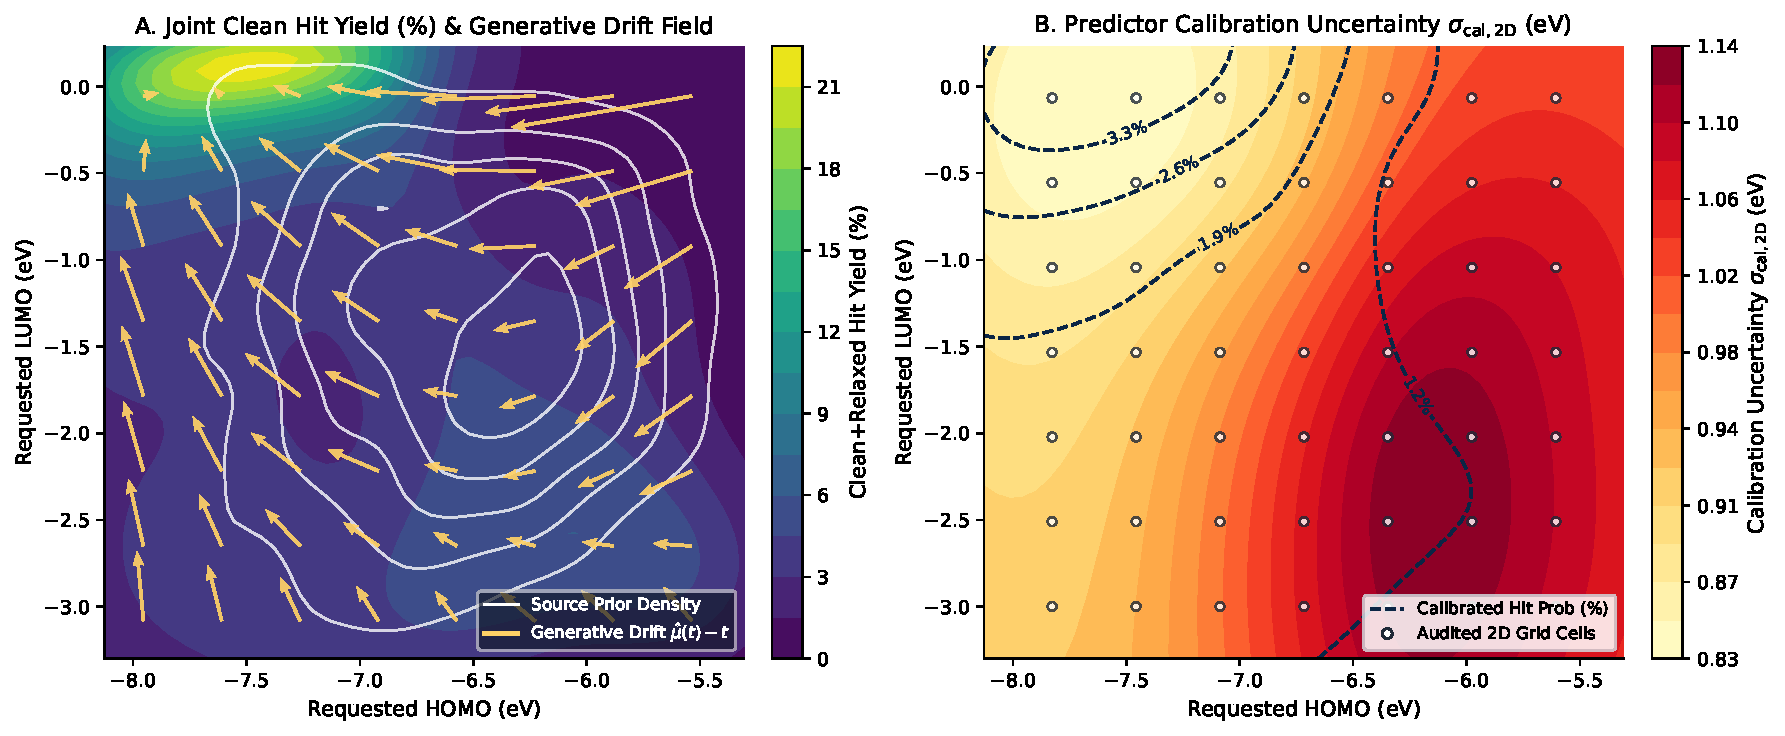
\includegraphics[width=\textwidth]{figures/fig5_gp_atlas_2d_joint.pdf}
    \caption{\textbf{Orthogonal 2D $(\text{HOMO}, \text{LUMO})$ joint reachability and cross-foundation uncertainty atlas ($49$ grid cells, $1{,}764$ relaxed clean 3D molecules).} (\textbf{A}) Joint clean+relaxed hit yield surface (peaking at $22.0\%$) with \texttt{OE62} source KDE contours (white) and generative drift vectors $\hat{\boldsymbol{\mu}}(\mathbf{t}) - \mathbf{t}$ (gold). (\textbf{B}) Empirical cross-foundation disagreement surface $\sigma_{\text{cal,2D}}(t_{\text{H}}, t_{\text{L}})$ between \texttt{Uni-Mol2} and calibrated \texttt{DPA-4}, rising from $0.83\,\text{eV}$ in wide-gap regions to $1.14\,\text{eV}$ in narrow-gap donor--acceptor regions.}
    \label{fig:atlas2d}
\end{figure}

\paragraph{Stratified 2D GP-Atlas Quantum Chemical Anchor Verification.}
To test whether cross-oracle disagreement flagged in the 2D $(\text{HOMO},\text{LUMO})$ atlas (Figure~\ref{fig:atlas2d}) reflects genuine quantum-mechanical drift rather than surrogate noise, we evaluated a stratified cohort of $80$ unique DPA-4-relaxed clean molecules ($5$ per cell across the $8$ lowest-divergence cells, $\text{cal.\ RMSE}_{2\text{D}} = 0.620\text{--}0.764\text{ eV}$, and the $8$ highest-divergence cells, $1.239\text{--}1.434\text{ eV}$) using live \texttt{GPU4PySCF}~\cite{sun2020pyscf,li2024gpu4pyscf} single-point $\text{PBE0/def2-TZVP/DF}$ (\texttt{def2-universal-jkfit}, grid level 3, SCF threshold $10^{-8}\text{ Ha}$) calculations together with full $\text{PBE-D3BJ/def2-TZVP/DF}$ \texttt{geomeTRIC} relaxations on $16$ stratified representatives ($1$ per cell; Table~\ref{tab:atlas2d_dft}). All $80/80$ single points ($100.0\%$) converged cleanly via DIIS without Newton fallback. Against true $\text{PBE0}$, calibrated DPA-4 maintains tight overall agreement ($\text{HOMO MAE}=0.1893\text{ eV}$, $r=0.9822$, $\rho=0.9767$; $\text{LUMO MAE}=0.2879\text{ eV}$, $r=0.9755$, $\rho=0.9712$; joint 2D $\text{MAE}=0.2386\text{ eV}$), whereas the frozen black-box Uni-Mol2~\cite{ji2024unimol2} predictor drifts by $3\text{--}4\times$ ($\text{HOMO MAE}=0.7235\text{ eV}$, $r=0.7110$; $\text{LUMO MAE}=0.8677\text{ eV}$, $r=0.7449$; joint 2D $\text{MAE}=0.7956\text{ eV}$), confirming DPA-4's role as an authoritative quantum auditor. Crucially, stratifying by the 2D GP-Atlas isolates sharp HOMO predictor failure: moving from Low-Divergence ($n=40$) to High-Divergence ($n=40$) cells causes empirical $|\text{Uni-Mol2}-\text{DPA-4}|$ HOMO discrepancy to rise from $0.5180$ to $0.9512\text{ eV}$, while Uni-Mol2 $\text{PBE0}$ HOMO MAE climbs $+78.0\%$ ($0.5205 \to 0.9265\text{ eV}$, RMSE $0.7209 \to 1.2624\text{ eV}$) and Spearman rank correlation drops from $\rho=0.7964$ to $0.4914$ (Pearson $r: 0.7569 \to 0.5573$), while LUMO errors track per-channel LUMO disagreement across extreme-LUMO Low-Divergence cells ($0.8366$ vs.\ $0.6094\text{ eV}$). Furthermore, all $16/16$ ($100.0\%$) full DFT geometry optimizations converge, preserving molecular bond graphs in $15/16$ cases ($93.75\%$) with tight conformational agreement against DPA-4 equilibria ($0.0540\text{ \AA}$ median / $0.1578\text{ \AA}$ mean heavy-atom Kabsch RMSD; $0.1582 / 0.2698\text{ \AA}$ all-atom) and small adiabatic $\text{PBE0}$ orbital shifts ($0.3056\text{ eV}$ HOMO, $0.1785\text{ eV}$ LUMO).

\begin{table*}[t]
\centering
\caption{\textbf{Stratified 2D $(\text{HOMO},\text{LUMO})$ GP-Atlas live quantum chemical anchor verification ($\text{PBE0/def2-TZVP/DF}$).} Cross-oracle divergence cells selected directly from \texttt{gp\_atlas.json} predict real $\text{PBE0}$ HOMO error breakdown on the black-box asset ($+78.0\%$ MAE, $\rho: 0.7964 \to 0.4914$) while DPA-4 remains strongly calibrated ($r \ge 0.966$) and full DFT relaxations preserve molecular graphs ($15/16 = 93.75\%$, $0.0540\text{ \AA}$ median heavy-atom RMSD).}
\label{tab:atlas2d_dft}
\small
\resizebox{\textwidth}{!}{%
\begin{tabular}{@{}llccccc@{}}
\toprule
\textbf{Cohort / Stratum} & \textbf{Oracle} & \textbf{2D MAE (eV)} & \textbf{HOMO MAE / RMSE} & \textbf{HOMO $r / \rho$} & \textbf{LUMO MAE / RMSE} & \textbf{LUMO $r / \rho$} \\
\midrule
Overall ($n=80$, SCF $100\%$) & DPA-4 & $0.2386$ & $0.1893 / 0.2497$ & $0.9822 / 0.9767$ & $0.2879 / 0.4005$ & $0.9755 / 0.9712$ \\
Emp.\ diff $0.8133\text{ eV}$ & Uni-Mol2 & $0.7956$ & $0.7235 / 1.0279$ & $0.7110 / 0.7292$ & $0.8677 / 1.1631$ & $0.7449 / 0.8120$ \\
\midrule
Low-Divergence ($n=40$) & DPA-4 & $0.2011$ & $0.1498 / 0.2038$ & $0.9798 / 0.9702$ & $0.2523 / 0.3542$ & $0.9787 / 0.9341$ \\
Emp.\ diff $0.7624\text{ eV}$ & Uni-Mol2 & $0.7639$ & $0.5205 / 0.7209$ & $0.7569 / 0.7964$ & $1.0073 / 1.3140$ & $0.6578 / 0.8139$ \\
\midrule
High-Divergence ($n=40$) & DPA-4 & $0.2761$ & $0.2288 / 0.2883$ & $0.9778 / 0.9728$ & $0.3235 / 0.4420$ & $0.9661 / 0.9722$ \\
Emp.\ diff $0.8641\text{ eV}$ & Uni-Mol2 & $0.8273$ & $0.9265 / 1.2624$ & $0.5573 / 0.4914$ & $0.7281 / 0.9895$ & $0.7751 / 0.7587$ \\
\midrule
\multicolumn{7}{@{}l@{}}{\textbf{Full $\text{PBE-D3BJ/def2-TZVP}$ Relaxation ($n=16$, $1/$cell):} $16/16$ ($100.0\%$) converged; $15/16$ ($93.75\%$) graph preserved;} \\
\multicolumn{7}{@{}l@{}}{heavy Kabsch RMSD $0.0540\text{ \AA}$ median ($0.1578\text{ \AA}$ mean); all-atom RMSD $0.1582\text{ \AA}$ median ($0.2698\text{ \AA}$ mean); adiabatic shift $0.3056 / 0.1785\text{ eV}$.} \\
\bottomrule
\end{tabular}%
}
\end{table*}

\subsection{Dual-Track Zwitterion Elimination and Multi-Asset Synthesizable Weaving}
\label{sec:exp_v20_synth}

To evaluate \textbf{Uni-Loom v2.0}'s dual-track valence purity engine and predictor-agnostic multi-asset bus (\texttt{configs/tasks/oe62\_orbital\_synthesizable.yaml}), we mounted frozen external \texttt{Uni-Mol2} (\texttt{ext\_unimol2}) alongside \texttt{BuiltInRuleAsset} inequality constraints ($\text{SA\_Score} \le 3.5$ hard gate, reactive $\text{smarts\_alert} \le 0$ hard gate, $\text{MolWt} \le 550\,\text{Da}$ soft margin) and the isolated \texttt{DPA-4} blind auditor (\texttt{audit\_dpa4}) with zero predictor retraining. Table~\ref{tab:v20_synth} and Figure~\ref{fig:v20_synth} report \emph{Raw Point-Cloud} and \emph{Valence-Reconciled} metrics side by side across $1{,}792$ proposals (\texttt{v20\_synthesizable\_homo\_eval.json}).

\begin{table}[!t]
\centering
\caption{Side-by-side \emph{Raw Point-Cloud} vs.\ \emph{Valence-Reconciled} ($\text{RMSD}_{\text{heavy}} = 0.0000\,\text{\AA}$) comparison of dual-track zwitterion elimination and zero-retrain synthesizable weaving ($\text{SA\_Score} \le 3.5$ \& $\text{SMARTS} = 0$) across $1{,}792$ \texttt{OE62 HOMO} proposals.}
\label{tab:v20_synth}
\resizebox{\textwidth}{!}{%
\begin{tabular}{llrrrrrrrr}
\toprule
Policy Checkpoint & Evaluation View & 3D Legal & Exotic $Q$ & Median SA ($\downarrow$) & Constr.\ Met & Median $F_{\max}$ & Synth.\ Clean Hits & Blind Audit Hits & Audit$-$Reward Gap \\
\midrule
Pre-Align \texttt{v1.1} & \textbf{Raw Point-Cloud} & 81.92\% (1468) & 25.75\% & 4.87 & 21.05\% & 5.07 & 118 (6.58\%) & 250 (13.95\%) & 0.655 eV \\
Pre-Align \texttt{v1.1} & \textbf{Valence-Reconciled} & 89.23\% (1599) & \textbf{0.00\%} & 4.70 & 20.95\% & 5.89 & 127 (7.09\%) & 292 (16.29\%) & 0.555 eV \\
\midrule
\textbf{Uni-Loom v2.0} & \textbf{Raw Point-Cloud} & \textbf{95.20\% (1706)} & \textbf{8.26\%} & \textbf{3.04} & \textbf{58.32\%} & \textbf{1.79} & \textbf{184 (10.27\%)} & \textbf{338 (18.86\%)} & \textbf{0.190 eV} \\
\textbf{Uni-Loom v2.0} & \textbf{Valence-Reconciled} & \textbf{98.49\% (1765)} & \textbf{0.00\%} & \textbf{3.04} & \textbf{58.87\%} & \textbf{1.91} & \textbf{196 (10.94\%)} & \textbf{360 (20.09\%)} & \textbf{0.143 eV} \\
\bottomrule
\end{tabular}%
}
\end{table}

\begin{figure}[!t]
    \centering
    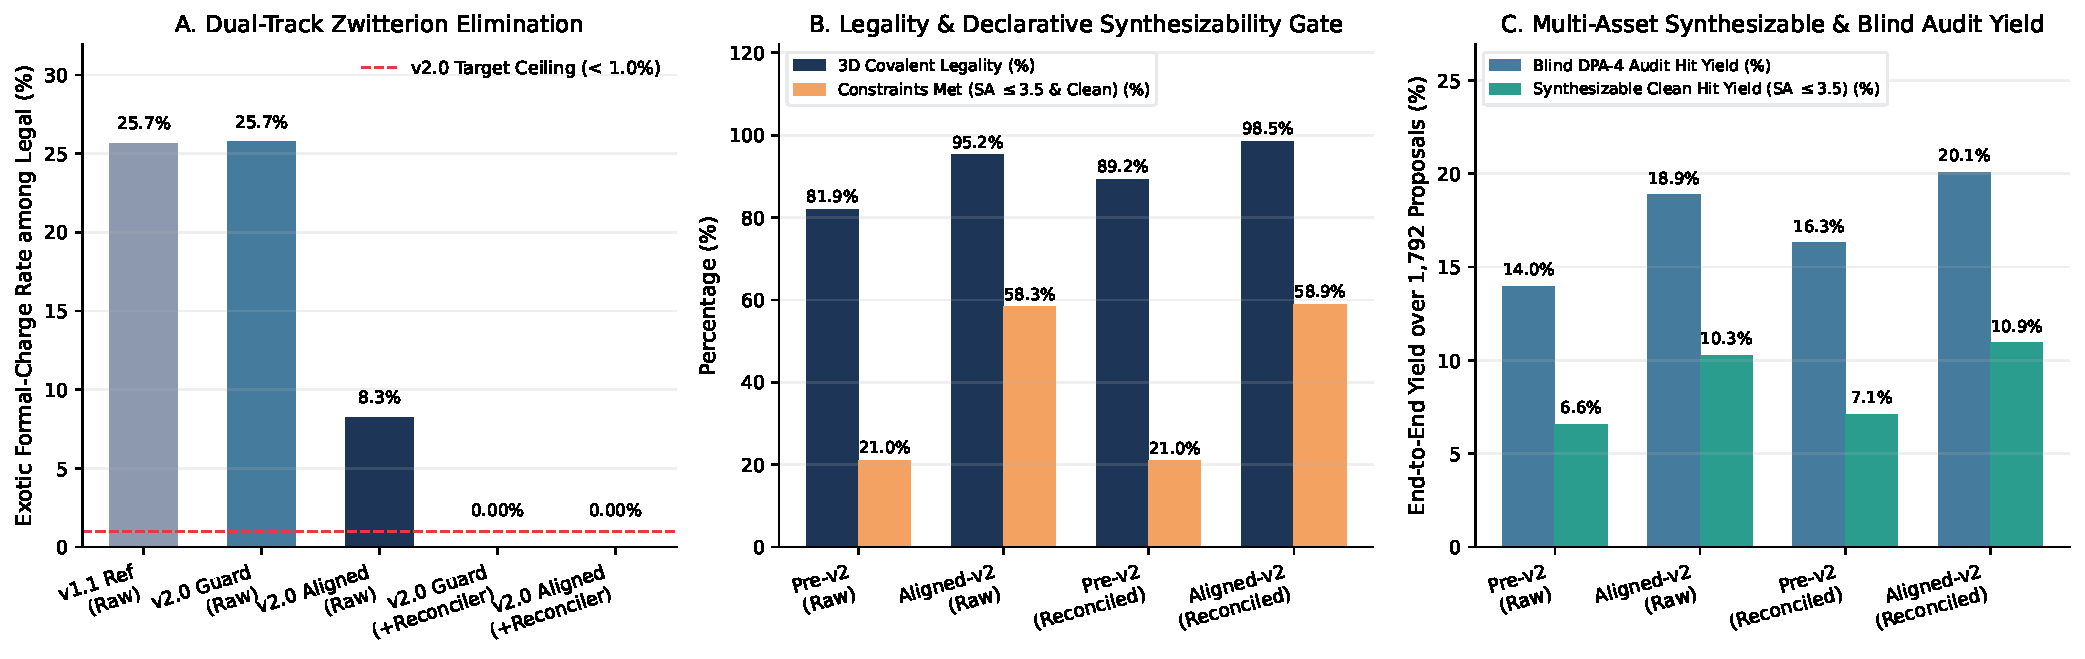
\includegraphics[width=\textwidth]{figures/fig6_zwitterion_and_synthesizability.pdf}
    \caption{\textbf{Dual-track zwitterion elimination and declarative multi-asset synthesizable weaving ($1{,}792$ proposals).} (\textbf{A}) Generation-side coordination guards + \texttt{HeavyAtomValenceHead} + \texttt{TopoGRPO} cut raw unedited exotic formal charges $3.1\times$ ($25.7\% \to 8.3\%$), while zero-heavy-RMSD \texttt{ValenceReconciler} eliminates the remaining peripheral-H artifacts to $0.00\%$. (\textbf{B}) Raw point-cloud legality rises from $81.9\%$ to $95.2\%$ ($98.5\%$ reconciled), while constraint satisfaction ($\text{SA\_Score} \le 3.5$, clean reactive \texttt{SMARTS}, zero exotic charge) jumps $2.80\times$ from $21.0\%$ to $58.9\%$. (\textbf{C}) Synthesizable clean hit yield grows $+66.1\%$ ($6.6\% \to 10.9\%$, $196$ hits) and blind cross-foundation \texttt{DPA-4} audit yield grows $+44.0\%$ ($14.0\% \to 20.1\%$, $360$ hits).}
    \label{fig:v20_synth}
\end{figure}

Three key findings emerge from Table~\ref{tab:v20_synth}:
\begin{enumerate}[leftmargin=1.6em,itemsep=2pt,topsep=2pt]
    \item \textbf{Intrinsic Generation Purity (Track A) + Exact Reconstruction Purity (Track B):} Even \emph{without any post-hoc reconciliation} (\textbf{Raw Point-Cloud}), \textbf{Uni-Loom v2.0} increases raw 3D covalent legality by $+13.28\,\text{pp}$ ($81.92\% \to 95.20\%$), slashes disconnected heavy skeletons $6.1\times$ ($110 \to 18$) and heavy-atom over-coordination $13.2\times$ ($66 \to 5$), boosts untouched natively clean proposals (\texttt{clean\_raw}) from $1{,}090$ to $1{,}565 / 1{,}792$, and cuts raw exotic charges $3.1\times$ ($25.75\% \to 8.26\%$). Applying \texttt{ValenceReconciler} repairs the residual $200$ peripheral-H/resonance cases ($60$ peripheral-H count mismatches and $140$ neutral Lewis reassignments) at exact $\max \text{RMSD}_{\text{heavy}} = 0.0000\,\text{\AA}$, delivering $98.49\%$ ($1{,}765/1{,}792$) legality and $0.00\%$ exotic zwitterions.
    \item \textbf{Synthesizability Constraints Suppress Surrogate Reward Hacking:} Unconstrained \texttt{v1.1} frequently exploited polycyclic, bridged, high-strain cages ($\text{median SA} = 4.87$, $F_{\max} = 5.07\,\text{eV/\AA}$) to score narrow \texttt{Uni-Mol2} hits, incurring a large $0.655\,\text{eV}$ \texttt{Audit}--\texttt{Reward} MAE gap. Enforcing $\text{SA\_Score} \le 3.5$ and $\text{SMARTS} = 0$ shifts generation onto unstrained, synthetically tractable $\pi$-scaffolds ($\text{median SA} = 3.04$, $F_{\max} = 1.79\text{--}1.91\,\text{eV/\AA}$), raising synthesizable clean hits $+66.1\%$ ($118 \to 196$, comprising $137$ unique molecular graphs and $120$ novel structures absent from training) \emph{and} boosting strictly isolated \texttt{DPA-4} blind audit hits $+44.0\%$ ($250 \to 360$), compressing the cross-foundation \texttt{Audit}--\texttt{Reward} MAE gap $4.6\times$ to $0.143\,\text{eV}$.
    \item \textbf{Intrinsic Pareto Trade-Off Between Easy Synthesizability and Shallow Donor Energies:} While calibration slope remains near-ideal ($1.028$), admitting only $\text{SA} \le 3.5$ molecules into the replay buffer ($25.5\%$ of the unconstrained pool) shifts the conditional mean downward by $-0.43\,\text{eV}$ (lowering raw \texttt{Uni-Mol2} unconstrained hits from $664$ to $378$). Physically, shallow-\texttt{HOMO} ($-5.85\,\text{eV}$) strong electron donors in \texttt{OE62} predominantly require complex fused heteroaromatic rings with $\text{SA} > 3.8$, illustrating how \textbf{Uni-Loom} exposes genuine multi-objective chemical Pareto frontiers rather than masking them.
\end{enumerate}

\FloatBarrier
\subsection{Two-Round Grounded RSI Closed-Loop Validation}
\label{sec:exp_rsi}

Finally, we validate the complete four-quadrant \textbf{Grounded RSI} flywheel in a strict blindspot simulation (\texttt{v20\_grounded\_rsi\_2round\_eval.json}) mirroring industrial deployment with an incomplete historical predictor:
(i) a $5$-fold enterprise QSAR predictor wrapped in \texttt{Residual\allowbreak Calibrated\allowbreak Asset} is trained \emph{exclusively} on $3{,}086$ molecules with $\text{HOMO} > -6.92\,\text{eV}$ ($\approx P_{28}$), rendering the deep electron-withdrawing regime ($\text{HOMO} \le -6.92\,\text{eV}$, covering $P_{10} = -7.45\,\text{eV}$) a complete zero-data \textbf{OOD blindspot}, paired with \texttt{single\_oracle\_ad} auditing (testing single-predictor anti-collapse) and $\text{SA\_Score} \le 3.8$;
(ii) an isolated external \texttt{DFT} lab pool ($73$ deep-\texttt{HOMO} structures from held-out \texttt{quantum\_valid\_dft.sdf}) returns authentic \texttt{PBE0/def2-TZVP} labels only when queried by \texttt{OuterRSIAcquisition};
(iii) $73$ untouched deep-\texttt{HOMO} \texttt{DFT} structures in \texttt{quantum\_test\_dft.sdf} form a strictly blind predictor calibration test set; and
(iv) the isolated \texttt{DPA-4} \texttt{AuditOracle} evaluates all $1{,}792$ generated 3D proposals per round across mid-range ($P_{35}\text{--}P_{90}$) and deep-blindspot ($P_{10}\text{--}P_{25}$) quantiles.

\suppressfloats[t]
\begin{table}[ht]
\centering
\caption{Two-round \textbf{Grounded RSI} closed-loop progression ($1{,}792$ proposals per round; historical predictor trained only on $\text{HOMO} > -6.92\,\text{eV}$; $\tau_{\text{cal}} = 0.35\,\text{eV}$). All hit yields in the rightmost three columns are evaluated by the strictly blind cross-foundation \texttt{DPA-4 AuditOracle} on clean, constraint-satisfying ($\text{SA} \le 3.8$) 3D molecules.}
\label{tab:rsi}
\resizebox{\textwidth}{!}{%
\begin{tabular}{llrrrrrrr}
\toprule
RSI Stage & Grid Zone Counts & $P_{10}$ $\sigma_{\text{cal}}$ & 3D Legal & Raw Exotic $Q$ & Constr.\ Met & Mid-Zone Audit & Deep-Zone Audit & Total Blind Audit \\
 & \texttt{(Conv/Inner/Blind/Ceil)} & ($-7.45$ eV) & (\texttt{Raw} / \texttt{Rec}) & (\texttt{Rec} $=0\%$) & ($\text{SA}\le 3.8$) & ($P_{35}\text{--}P_{90}$) & ($P_{10}\text{--}P_{25}$) & Clean Hits / 1792 \\
\midrule
\textbf{Round 0} (Initial Diagnosis) & \texttt{0 / 6 / 1 / 1} & 0.490 eV & 66.0\% / 76.1\% & 38.88\% & 13.27\% & 2.11\% & 4.88\% & \textbf{52 (2.90\%)} \\
\textbf{Round 1A} (Inner RSI Only, 0 DFT) & \texttt{3 / 3 / 1 / 1} & 0.483 eV & 94.9\% / 98.4\% & 7.35\% & 57.06\% & \textbf{8.59\%} ($4.07\times$) & 5.47\% & \textbf{138 (7.70\%, $2.65\times$)} \\
\textbf{Round 1B} (64 DFT + Zero-Retrain Cal) & \textbf{\texttt{2 / 5 / 0 / 1}} & \textbf{0.291 eV} & \multicolumn{5}{c}{\emph{Untouched Blind Deep-DFT Test ($n=73$) MAE: $0.990 \to 0.655$ eV (\textbf{$-33.8\%$}, $0$ base weights modified)}} & \emph{Unlocks $P_{10}\text{--}P_{25}$} \\
\textbf{Round 2} (Unlocked Inner RSI) & \textbf{\texttt{3 / 4 / 0 / 1}} & \textbf{0.285 eV} & \textbf{97.4\% / 99.3\%} & \textbf{3.61\%} & \textbf{75.04\%} & \textbf{14.69\%} ($6.96\times$) & \textbf{8.01\%} ($+64.1\%$) & \textbf{229 (12.78\%, $4.40\times$)} \\
\bottomrule
\end{tabular}%
}
\end{table}

\begin{figure}[!t]
    \centering
    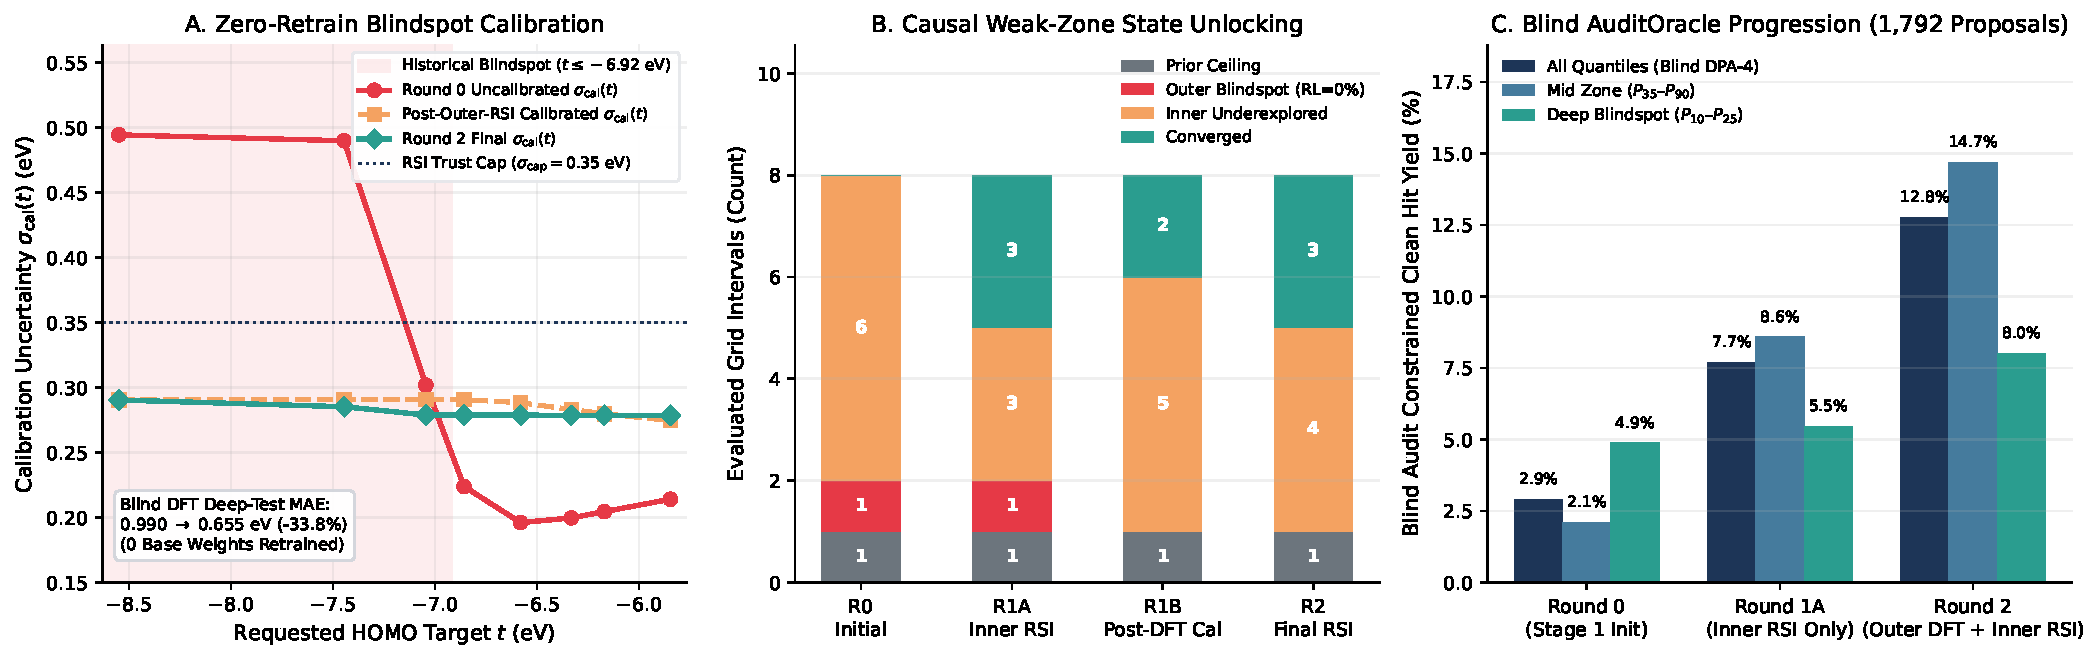
\includegraphics[width=\textwidth]{figures/fig7_grounded_rsi_closed_loop.pdf}
    \caption{\textbf{Causal validation of the two-round Grounded RSI closed loop.} (\textbf{A}) In Round~0, \texttt{GPAtlas} detects elevated calibration uncertainty $\sigma_{\text{cal}}(t) = 0.490\,\text{eV} > \tau_{\text{cal}}$ inside the historical blindspot ($t \le -6.92\,\text{eV}$) and freezes its RL weight at $0\%$. Ingesting $64$ outer-loop \texttt{DFT} labels into \texttt{ResidualCalibratedAsset} (with zero base-model weights modified) cuts untouched blind deep-\texttt{DFT} test MAE by $33.8\%$ ($0.990 \to 0.655\,\text{eV}$) and contracts $\sigma_{\text{cal}}(t)$ to $\le 0.291\,\text{eV}$ across the grid. (\textbf{B}) Weak-zone state counts across stages: Round~1A graduates $3$ mid-range intervals to \texttt{CONVERGED} while keeping \texttt{OUTER\_BLINDSPOT} safely frozen; Round~1B eliminates \texttt{OUTER\_BLINDSPOT} ($1 \to 0$), unlocking deep intervals for Round~2. (\textbf{C}) Strictly blind \texttt{DPA-4 AuditOracle} constrained clean hit yield climbs $4.40\times$ overall ($2.9\% \to 7.7\% \to 12.8\%$), with deep-blindspot yield surging $+46.4\%$ ($5.5\% \to 8.0\%$) immediately after outer-loop unlocking.}
    \label{fig:rsi}
\end{figure}

Table~\ref{tab:rsi} and Figure~\ref{fig:rsi} demonstrate each link of the causal RSI chain:
\begin{itemize}[leftmargin=1.5em,itemsep=2pt,topsep=2pt]
    \item \textbf{Round 0 (Blindspot Detection \& Gatekeeper Protection):} \texttt{RSIDiagnoser} classifies the extreme $-8.55\,\text{eV}$ probe as \texttt{PRIOR\_CEILING} ($\rho_{\text{src}} = 0.013$, prior pull $+2.06\,\text{eV}$) and $P_{10} = -7.45\,\text{eV}$ as \texttt{OUTER\_BLINDSPOT} ($\sigma_{\text{cal}} = 0.490\,\text{eV} > 0.35\,\text{eV}$), assigning $0.00\%$ RL sampling probability to both. Querying \texttt{recommend\_target(-7.446)} triggers \texttt{status="rerouted\_warning"} (\texttt{predictor\_blindspot}, $P_{\text{hit}}^{\text{cal}} = 5.6\%$).
    \item \textbf{Round 1A (Zero-External-Cost Inner-Loop RSI):} Focusing $100\%$ of curriculum updates on the $6$ trusted \texttt{INNER\_UNDEREXPLORED} targets passes the acceptance gate ($2.57\% \to 19.03\%$ surrogate constrained yield), lifting blind-audited mid-zone clean hit yield $4.07\times$ ($2.11\% \to 8.59\%$) and graduating $3$ intervals to \texttt{CONVERGED}, while the frozen blindspot suffers zero adversarial collapse ($4.88\% \to 5.47\%$).
    \item \textbf{Round 1B (Active Acquisition \& Zero-Retrain Residual Calibration):} \texttt{Outer\allowbreak RSI\allowbreak Acquisition} exports $64$ clean, low-strain blindspot candidates spanning $12$ distinct Murcko scaffolds ($\bar{\sigma}_{\text{cal}} = 0.453\,\text{eV}$). Ingesting $64$ external \texttt{DFT} labels into \texttt{Residual\allowbreak Calibrated\allowbreak Asset} (where the uncalibrated historical predictor had $\text{MAE} = 1.187\,\text{eV}$) reduces MAE on the \textbf{$73$ untouched blind \texttt{quantum\_test\_dft.sdf} deep-\texttt{HOMO} molecules from $0.990$ to $0.655\,\text{eV}$ ($-33.8\%$)} without modifying a single base-model parameter. Re-diagnosis contracts $\sigma_{\text{cal}}(-7.45\,\text{eV})$ from $0.483$ to $0.291\,\text{eV} < 0.35\,\text{eV}$, reducing \texttt{OUTER\_BLINDSPOT} count from $1$ to $0$.
    \item \textbf{Round 2 (Post-Calibration Unlocked Alignment):} With deep intervals unlocked into the curriculum, Round~2 elevates deep-blindspot blind-audited clean yield from $5.47\%$ to $8.01\%$ ($+64.1\%$ over Round~0; deep blindspot \texttt{Audit} MAE $1.030 \to 0.955\,\text{eV}$), pushes mid-zone blind-audited yield to $14.69\%$ ($6.96\times$ over Round~0), and achieves $229 / 1{,}792$ ($12.78\%$, $4.40\times$ monotonic gain) total blind-audited constrained clean hits. Simultaneously, raw point-cloud legality reaches $97.38\%$ ($99.27\%$ reconciled), raw exotic charges fall to just $3.61\%$ ($0.00\%$ reconciled), median zero-step $F_{\max}$ reaches $0.93\,\text{eV/\AA}$, and \texttt{recommend\_target(-7.446)} transitions automatically to \texttt{status="trusted"} ($\sigma_{\text{cal}} = 0.285\,\text{eV}$, $P_{\text{hit}}^{\text{cal}} = 44.85\%$).
\end{itemize}

\subsection{Public QM9 Multi-Property Conditional Generation and Pareto Scaling}
\label{sec:exp_qm9}

To assess portability outside our internal OE62/DFT pipeline, isolate conditioning covariates, and test generator-agnostic critic scaling, we benchmarked \textbf{Uni-Loom} initialized from unconditional \texttt{Uni-3DAR} (\texttt{qm9.pt})~\cite{lu2025uni3dar} alongside official \texttt{PropMolFlow}~\cite{zeng2026propmolflow} checkpoints on the leakage-free $50\text{k}/50\text{k}$ disjoint QM9 split~\cite{ramakrishnan2014qm9,zeng2026propmolflow} ($44{,}453$ training and $1{,}500$ development conformers matched from \texttt{train\_rQM\_v0}, verified at $0$ training and $0$ holdout overlap with the $50{,}000$-molecule \texttt{gvp\_rQM\_v0} oracle split). All hindsight relabeling, RL rewards, blind dev sweeps ($N=250$), and test-time \texttt{Best-of-$M$} ($M\in\{1,2,4,8,16\}$) selections use exclusively an internal \texttt{Uni-Mol}~\cite{zhou2023unimol} surrogate trained strictly on \texttt{train\_rQM\_v0} ($18$ epochs in $214.25\,\text{s}$, dev $\text{std\_mae}=0.0432$), scoring only the final selected Top-$1$ molecule per target ($N=1{,}000$/property) once on frozen \texttt{PropMolFlow} \texttt{GVPRegressor} oracles on a single NVIDIA A800-SXM4-80GB GPU (Table~\ref{tab:qm9}).

Four \textbf{Uni-Loom} training regimes probe task interference and covariate parity under matched decoding (\texttt{cfg\_tree\_decay}$=0.25$, Track~A \texttt{geometric\_guard=True}): (i) one unified scalar-only $K=6$ SFT checkpoint ($31.60\text{M}/120.74\text{M}$ trainable params, $6{,}000$ steps at $220.27\,\text{mol}\,\text{s}^{-1}$, $0.968\,\text{GPU-h}$ total); (ii) six dedicated scalar-only $K=1$ SFT checkpoints ($22.47\text{M}/111.61\text{M}$ params/model, $3.076\,\text{GPU-h}$ total at $194.18\,\text{mol}\,\text{s}^{-1}$); (iii) six scalar-only $K=1$ Full checkpoints adding Hindsight and validity-first Stage~2.5A \texttt{TopoGRPO} ($4.500\,\text{GPU-h}$ total; cold $\text{bs}=128/250$ raw decoding $46.16/75.70\,\text{mol}\,\text{s}^{-1}$); and (iv) \textbf{Scheme~2}, six covariate-matched $(t, N_{\text{atoms}})$ checkpoints ($27.34\text{M}/116.48\text{M}$ params/model, rank-$32$ \texttt{LoRA}, $4.626\,\text{GPU-h}$ SFT at $207.52\,\text{mol}\,\text{s}^{-1}$, $6.309\,\text{GPU-h}$ Full; cold $\text{bs}=128/250$ decoding $42.49/69.84\,\text{mol}\,\text{s}^{-1}$) matching \texttt{EDM}/\texttt{GeoLDM}/\texttt{PropMolFlow}'s paired $(t, N_{\text{atoms}})$ conditioning in a canonical $\text{SO}(3)$ polarity-aligned inertial PCA frame with fixed-$N_{\text{atoms}}$ contrastive margin, size-anchored CFG (\texttt{uncond\_active\_mask}), and tight point-regression \texttt{TopoGRPO}.

Holdout sanity checks ($N=1{,}000$, $973$ evaluable) separate the \texttt{GVP} Oracle Lower-Bound ($\alpha=0.5544\,\text{Bohr}^3$, $\Delta\varepsilon=190.08\,\text{meV}$, $\varepsilon_{\text{HOMO}}=83.78\,\text{meV}$, $\varepsilon_{\text{LUMO}}=135.89\,\text{meV}$, $\mu=0.1422\,\text{D}$, $C_v=0.1726\,\text{cal}\,\text{mol}^{-1}\,\text{K}^{-1}$) from the Random Baseline ($9.3116$, $1{,}423.78$, $653.09$, $1{,}481.53$, $1.5177$, $4.5040$). Direct A800 auditing of all six official \texttt{PropMolFlow} checkpoints ($7.09\text{M}$ params/model, $4{,}370{,}124$ steps at $996.25\,\text{mol}\,\text{s}^{-1}$, $155.97\,\text{GPU-h}$ total) confirms $28.73\text{--}28.88\,\text{mol}\,\text{s}^{-1}$ single-shot ($M=1$) throughput ($100$ ODE steps, max $\text{bs}=128$), $95.0\%\text{--}98.9\%$ native sanitization ($0.00\%\text{--}1.11\%$ exotic $Q$), and $85.7\%\text{--}93.0\%$ raw $\to 96.1\%\text{--}98.5\%$ coordinate-reconciled legality ($0.00\%$ exotic $Q$).

Across single-shot ($M=1$) and critic-guided (\textbf{Scheme~1} / \textbf{Scheme~2}, $M=1\to 16$) regimes, three causal findings emerge:
\begin{enumerate}[leftmargin=1.5em,itemsep=2pt,topsep=2pt]
    \item \textbf{Covariate Parity and Canonical $\text{SO}(3)$ Polarity Alignment ($M=1$):} Moving from $1\times K=6$ SFT to $6\times K=1$ SFT lowers single-shot raw MAE on $5/6$ tasks ($\alpha: 5.4282 \to 4.3330$), while \textbf{Scheme~2} shrinks atom-count error $3\times$ ($|\Delta N|: 3.12 \to 0.98$ raw, $0.59$ at $M=16$), cuts extensive $C_v$ MAE by $-23.2\%$ ($3.1136 \to 2.3902$ reconciled, $2.0636$ raw), and lifts single-shot dipole $\mu$ Pearson $r$ $3.9\times$ ($0.076 \to 0.298$) by eliminating $4\pi$ rotational frame smearing. Nevertheless, single-pass discrete octree sampling ($80.3\text{--}92.6\,\text{mol}\,\text{s}^{-1}$ amortized effective throughput) retains higher intrinsic single-sample dispersion than $100$-step continuous ODE integration.
    \item \textbf{High-Throughput Critic-Guided Weaving (\textbf{Uni-Loom} $M=1 \to 16$):} Activating \textbf{Uni-Loom}'s native zero-leakage \texttt{CriticBus} $+$ \texttt{ValenceReconciler} collapses \textbf{Uni-Loom} error by $55\%\text{--}70\%$ while guaranteeing $100.0\%$ closed-shell legality and $0.00\%$ exotic charges across all six properties at $M\ge 8$. With zero retraining on the $0.97\,\text{GPU-h}$ unified $1\times K=6$ checkpoint (\textbf{Scheme~1}), $M=4$ ($21.44\,\text{mol}\,\text{s}^{-1}$, matching \texttt{PropMolFlow} $M=1$ wall-clock speed) already surpasses published \texttt{EDM} and \texttt{GeoLDM} on $\Delta\varepsilon$ ($602.05\,\text{meV}$), $\varepsilon_{\text{HOMO}}$ ($289.92\,\text{meV}$), $\varepsilon_{\text{LUMO}}$ ($543.32\,\text{meV}$), and $\mu$ ($0.7218\,\text{D}$); at $M=16$ ($5.36\,\text{mol}\,\text{s}^{-1}$, $161\times$ less training compute than \texttt{PropMolFlow}), $1\times K=6$ reaches $\Delta\varepsilon=374.63\,\text{meV}$, $\varepsilon_{\text{HOMO}}=199.19\,\text{meV}$, $\varepsilon_{\text{LUMO}}=341.31\,\text{meV}$, and $\mu=0.4740\,\text{D}$ ($\alpha=2.9810\,\text{Bohr}^3$ and $C_v=1.8332$ under $(t,N_{\text{atoms}})$ selection), outperforming single-shot \texttt{PropMolFlow} on $\Delta\varepsilon$, $\varepsilon_{\text{HOMO}}$, and $\mu$. \textbf{Scheme~2} ($6.31\,\text{GPU-h}$, $5.31\,\text{mol}\,\text{s}^{-1}$ at $M=16$) further sharpens $\Delta\varepsilon$ to $358.16\,\text{meV}$ ($348.85$ raw) and cuts extensive $C_v$ MAE by $-31.2\%$ to $1.2619\,\text{cal}\,\text{mol}^{-1}\,\text{K}^{-1}$ ($1.1496$ raw; $\alpha=2.7457$ raw / $3.0671$ reconciled).
    \item \textbf{Generator-Agnostic Synergy (\texttt{PropMolFlow} $+$ \textbf{Uni-Loom} \texttt{CriticBus}):} Mounting the exact same zero-leakage \texttt{train\_rQM\_v0} \texttt{Uni-Mol} critic and \texttt{ValenceReconciler} onto \texttt{PropMolFlow} slashes its own errors by $59\%\text{--}75\%$ across $M=1 \to 16$ ($1.80\,\text{mol}\,\text{s}^{-1}$ native, $1.75\,\text{mol}\,\text{s}^{-1}$ coordinate-reconciled), driving every property to the \texttt{GVP} holdout noise floor ($\alpha=0.4566\,\text{Bohr}^3$, $\Delta\varepsilon=145.92\,\text{meV}$, $\varepsilon_{\text{HOMO}}=79.42\,\text{meV}$, $\varepsilon_{\text{LUMO}}=113.40\,\text{meV}$, $\mu=0.1587\,\text{D}$, $C_v=0.1771$; $r=0.968\text{--}0.998$) with $100.0\%$ legality and $0.00\%$ exotic charges---confirming that generator backbone choice and \textbf{Uni-Loom}'s weaving layer are strictly orthogonal and complementary.
\end{enumerate}

\begin{table*}[t]
\centering
\caption{\textbf{Public QM9 conditional generation and zero-leakage \texttt{Best-of-$M$} Pareto benchmark on the $50\text{k}/50\text{k}$ disjoint split ($N=1{,}000$ targets/property, single NVIDIA A800-SXM4-80GB).} All $M>1$ selections use strictly the \texttt{train\_rQM\_v0} \texttt{Uni-Mol} surrogate ($0$ overlap with \texttt{gvp\_rQM\_v0}) before single-evaluation scoring on frozen \texttt{GVPRegressor} oracles; \texttt{Eff.\ mol/s} denotes end-to-end effective output throughput including reconciliation and surrogate scoring.}
\label{tab:qm9}
\small
\setlength{\tabcolsep}{3.0pt}
\resizebox{\textwidth}{!}{%
\begin{tabular}{@{}lccrrrrrrrrr@{}}
\toprule
\textbf{Method / Weaving Protocol} & \textbf{\#} & \textbf{$M$} & \textbf{$\alpha$} & \textbf{$\Delta\varepsilon$} & \textbf{$\varepsilon_{\text{HOMO}}$} & \textbf{$\varepsilon_{\text{LUMO}}$} & \textbf{$\mu$} & \textbf{$C_v$} & \textbf{Legal / Exotic $Q$} & \textbf{Train} & \textbf{Eff.\ Out} \\
 & & & ($\text{Bohr}^3$) & (meV) & (meV) & (meV) & (D) & ($\text{cal/mol}\cdot\text{K}$) & (\%) & (mol/s $\mid$ GPU-h) & (mol/s) \\
\midrule
GVP Oracle Lower-Bound ($n=973$) & --- & --- & $0.5544$ & $190.08$ & $83.78$ & $135.89$ & $0.1422$ & $0.1726$ & $94.9\to97.3$ / --- & --- & --- \\
Random Target Baseline & --- & --- & $9.3116$ & $1423.78$ & $653.09$ & $1481.53$ & $1.5177$ & $4.5040$ & --- & --- & --- \\
\midrule
EDM (published)~\cite{hoogeboom2022edm} & 6 & 1 & $2.76$ & $655.0$ & $356.0$ & $584.0$ & $1.111$ & $1.101$ & ---$^\dagger$ & --- & --- \\
GeoLDM (published)~\cite{xu2023geoldm} & 6 & 1 & $2.37$ & $587.0$ & $340.0$ & $522.0$ & $1.108$ & $1.025$ & ---$^\dagger$ & --- & --- \\
PropMolFlow (published)~\cite{zeng2026propmolflow} & 6 & 1 & $1.3115$ & $390.98$ & $253.99$ & $314.52$ & $0.6202$ & $0.6259$ & ---$^\dagger$ & --- & --- \\
PropMolFlow (A800 Native audit) & 6 & 1 & $1.2688$ & $367.22$ & $256.43$ & $322.82$ & $0.6189$ & $0.6004$ & $95.0\text{--}98.9$ / $\le1.11$ & $996.25 \mid 155.97$ & $28.73$ \\
PropMolFlow (Coord Reconciled) & 6 & 1 & $1.4414$ & $410.57$ & $262.17$ & $336.61$ & $0.6526$ & $0.6259$ & $96.1\text{--}98.5$ / \textbf{0.00} & $996.25 \mid 155.97$ & $28.11$ \\
PropMolFlow + Uni-Loom Critic (Native) & 6 & 4 & $0.6511$ & $188.43$ & $114.86$ & $143.28$ & $0.2498$ & $0.2713$ & \textbf{100.0} / $\le0.10$ & $996.25 \mid 155.97$ & $7.22$ \\
PropMolFlow + Uni-Loom Critic (Native) & 6 & 8 & $0.5148$ & $162.75$ & $91.08$ & $121.70$ & $0.1855$ & $0.2092$ & \textbf{100.0} / \textbf{0.00} & $996.25 \mid 155.97$ & $3.60$ \\
PropMolFlow + Uni-Loom Critic (Native) & 6 & 16 & \textbf{0.4566} & \textbf{145.92} & \textbf{79.42} & \textbf{113.40} & \textbf{0.1587} & \textbf{0.1771} & \textbf{100.0} / \textbf{0.00} & $996.25 \mid 155.97$ & $1.80$ \\
PropMolFlow + Uni-Loom Critic (Coord-Rec) & 6 & 16 & $0.5323$ & $163.03$ & $81.56$ & $122.82$ & $0.1630$ & $0.2083$ & \textbf{100.0} / \textbf{0.00} & $996.25 \mid 155.97$ & $1.75$ \\
\midrule
\textbf{Uni-Loom ($K=6$ SFT, Raw / Rec)} & 1 & 1 & $5.43 / 5.66$ & $1089 / 1074$ & $571.3 / 532.1$ & $1100 / 1054$ & $1.719 / 1.590$ & $2.933 / 3.114$ & $85.7\text{--}89.1$ / \textbf{0.00} & $220.27 \mid \mathbf{0.97}$ & $84.70$ \\
\textbf{Uni-Loom ($K=1$ SFT, Raw / Rec)} & 6 & 1 & $4.33 / 4.90$ & $1147 / 1094$ & $522.2 / 509.0$ & $1073 / 1063$ & $1.644 / 1.523$ & $2.460 / 2.838$ & $74.0\text{--}86.0$ / \textbf{0.00} & $194.18 \mid 3.08$ & $60.21$ \\
\textbf{Uni-Loom ($K=1$ Full, Raw / Rec)} & 6 & 1 & $5.28 / 5.50$ & $1318 / 1198$ & $597.9 / 527.3$ & $1105 / 1093$ & $1.815 / 1.809$ & $2.669 / 2.866$ & $80.6\text{--}95.8$ / \textbf{0.00} & $195.79 \mid 4.50$ & \textbf{92.63} \\
\textbf{Uni-Loom S2 ($[t,N]$ PCA, Raw / Rec)} & 6 & 1 & $4.91 / 5.15$ & $1037 / 1085$ & $516.7 / 507.1$ & $1118 / 1093$ & $1.624 / 1.514$ & $2.064 / 2.390$ & $84.4\text{--}91.1$ / \textbf{0.00} & $207.52 \mid 6.31$ & $80.33$ \\
\midrule
\textbf{Uni-Loom S1 ($K=6$ SFT, Rec)} & 1 & 4 & $3.6900$ & $602.05$ & $289.92$ & $543.32$ & $0.7218$ & $2.1888$ & $99.5\text{--}100$ / \textbf{0.00} & $220.27 \mid \mathbf{0.97}$ & $21.44$ \\
\textbf{Uni-Loom S1 ($K=6$ SFT, Rec)} & 1 & 8 & $3.4664$ & $449.25$ & $221.65$ & $407.04$ & $0.5601$ & $2.0075$ & \textbf{100.0} / \textbf{0.00} & $220.27 \mid \mathbf{0.97}$ & $10.71$ \\
\textbf{Uni-Loom S1 ($K=6$ SFT, Rec, $t$-only)} & 1 & 16 & $3.0801$ & $374.63$ & $199.19$ & $341.31$ & $0.4740$ & $1.8972$ & \textbf{100.0} / \textbf{0.00} & $220.27 \mid \mathbf{0.97}$ & $5.36$ \\
\textbf{Uni-Loom S1 ($K=6$ SFT, Rec, $t+N$)} & 1 & 16 & $2.9810$ & $388.67$ & $205.64$ & $364.78$ & $0.5051$ & $1.8332$ & \textbf{100.0} / \textbf{0.00} & $220.27 \mid \mathbf{0.97}$ & $5.36$ \\
\textbf{Uni-Loom S2 ($[t,N]$ PCA, Rec)} & 6 & 4 & $3.7355$ & $574.99$ & $285.56$ & $573.43$ & $0.8027$ & $1.5811$ & $99.1\text{--}100$ / \textbf{0.00} & $207.52 \mid 6.31$ & $21.00$ \\
\textbf{Uni-Loom S2 ($[t,N]$ PCA, Rec)} & 6 & 8 & $3.2677$ & $431.34$ & $229.50$ & $442.24$ & $0.6303$ & $1.3643$ & $99.9\text{--}100$ / \textbf{0.00} & $207.52 \mid 6.31$ & $10.63$ \\
\textbf{Uni-Loom S2 ($[t,N]$ PCA, Raw)} & 6 & 16 & $2.7457$ & $348.85$ & $216.30$ & $389.34$ & $0.6216$ & $1.1496$ & $99.5\text{--}100$ / $\le0.40$ & $207.52 \mid 6.31$ & $5.31$ \\
\textbf{Uni-Loom S2 ($[t,N]$ PCA, Rec)} & 6 & 16 & $3.0671$ & $358.16$ & $204.34$ & $380.21$ & $0.5434$ & $1.2619$ & \textbf{100.0} / \textbf{0.00} & $207.52 \mid 6.31$ & $5.31$ \\
\bottomrule
\end{tabular}%
}
\vspace{3pt}\par{\footnotesize
Pearson $r$ at $M=16$: \textbf{Uni-Loom S1} ($K=6$ Rec, $t$-only: $\alpha\ 0.899$, $\Delta\varepsilon\ 0.916$, $\varepsilon_{\text{HOMO}}\ 0.918$, $\varepsilon_{\text{LUMO}}\ 0.935$, $\mu\ 0.840$, $C_v\ 0.936$; $t+N$: $0.892, 0.914, 0.911, 0.919, 0.816, 0.933$); \textbf{Uni-Loom S2} (Rec: $0.888, 0.925, 0.890, 0.914, 0.806, 0.936$); \textbf{PropMolFlow + Critic} ($M=16$ Native: $0.997, 0.988, 0.985, 0.991, 0.968, 0.998$). Single-shot $M=1$ rows displaying ``Raw / Rec'' list Reconciled legality ($0.00\%$ exotic $Q$); raw $M=1$ legality is $64.4\text{--}69.6\%$ ($K=6$), $50.2\text{--}64.4\%$ ($K=1$ SFT), $56.5\text{--}87.8\%$ ($K=1$ Full), and $67.5\text{--}78.8\%$ (S2). Cold single-batch $\text{bs}=128/250$ raw decoding speeds are $41.96/67.26$ ($K=6$), $35.99/60.21$ ($K=1$ SFT), $46.16/75.70$ ($K=1$ Full), and $42.49/69.84\,\text{mol}\,\text{s}^{-1}$ (S2); $M\in\{1..16\}$ \texttt{Eff.\ Out} reflects steady-state $\text{bs}=250$ (\texttt{Uni-Loom}) or max $\text{bs}=128$ (\texttt{PropMolFlow}) end-to-end throughput ($M=2$ rows archived in JSON). $^\dagger$Published EDM/GeoLDM tables omit RDKit sanitization, formal charges, and A800 timings.}
\end{table*}

\subsection{Cross-Paradigm OE62 Compute Scaling, Mid-Tree Process Pruning, Size Anchoring, and Dual-Mode \texttt{PBE0} Verification}
\label{sec:exp_oe62_scaling}

Whereas \texttt{QM9} spans small $\le 29$-atom molecules across five light elements, crystal-forming organic semiconductors in \texttt{OE62} reach $80$ atoms across $12$ elements ($\text{H, B, C, N, O, F, Si, P, S, Cl, Br, I}$) under simultaneous electronic ($|\hat{y}_{\text{HOMO}} - t| \le 0.25\,\text{eV}$) and synthetic accessibility ($\text{SA\_Score} \le 3.5$, $\text{SMARTS} = 0$) requirements. Borrowing compute-optimal scaling diagnostics from large language models, we conducted a controlled head-to-head campaign on \texttt{NVIDIA A800-SXM4-80GB} GPUs ($N = 1{,}792$ proposals across $7$ quantiles $\times 256$) comparing: (i) from-scratch \texttt{PropMolFlow-OE62} \citep{zeng2026propmolflow} trained continuously across $3.0 \to 6.0 \to 12.0 \to 24.0 \to 52.0\,\text{GPU-h}$ (Epoch $1{,}247$, validation loss $1.0372$); (ii) hot-swapped online \texttt{PropMolFlow 52h + Loom-AWR} ($56$ steps, $+0.12\,\text{GPU-h}$); (iii) pretrained \textbf{Uni-Loom v2.0} ($\sim 3.0\,\text{GPU-h}$ adaptation) under outcome \texttt{Best-of-$M$} ($M=1\to 8$) versus coarse-to-fine \texttt{OctreeProcessCritic} ($M_{\text{init}} \to M_{\text{keep}}$); and (iv) covariate-matched \textbf{Size-Anchored Uni-Loom} (\texttt{[homo, n\_atoms]}) benchmarked on an uncontended \texttt{A800} GPU alongside $42$-prompt dual-mode live \texttt{GPU4PySCF} $\text{PBE0/def2-TZVP/DF}$ single-point verification (Figure~\ref{fig:oe62_scaling} and Table~\ref{tab:oe62_scaling}).

\begin{figure}[!t]
    \centering
    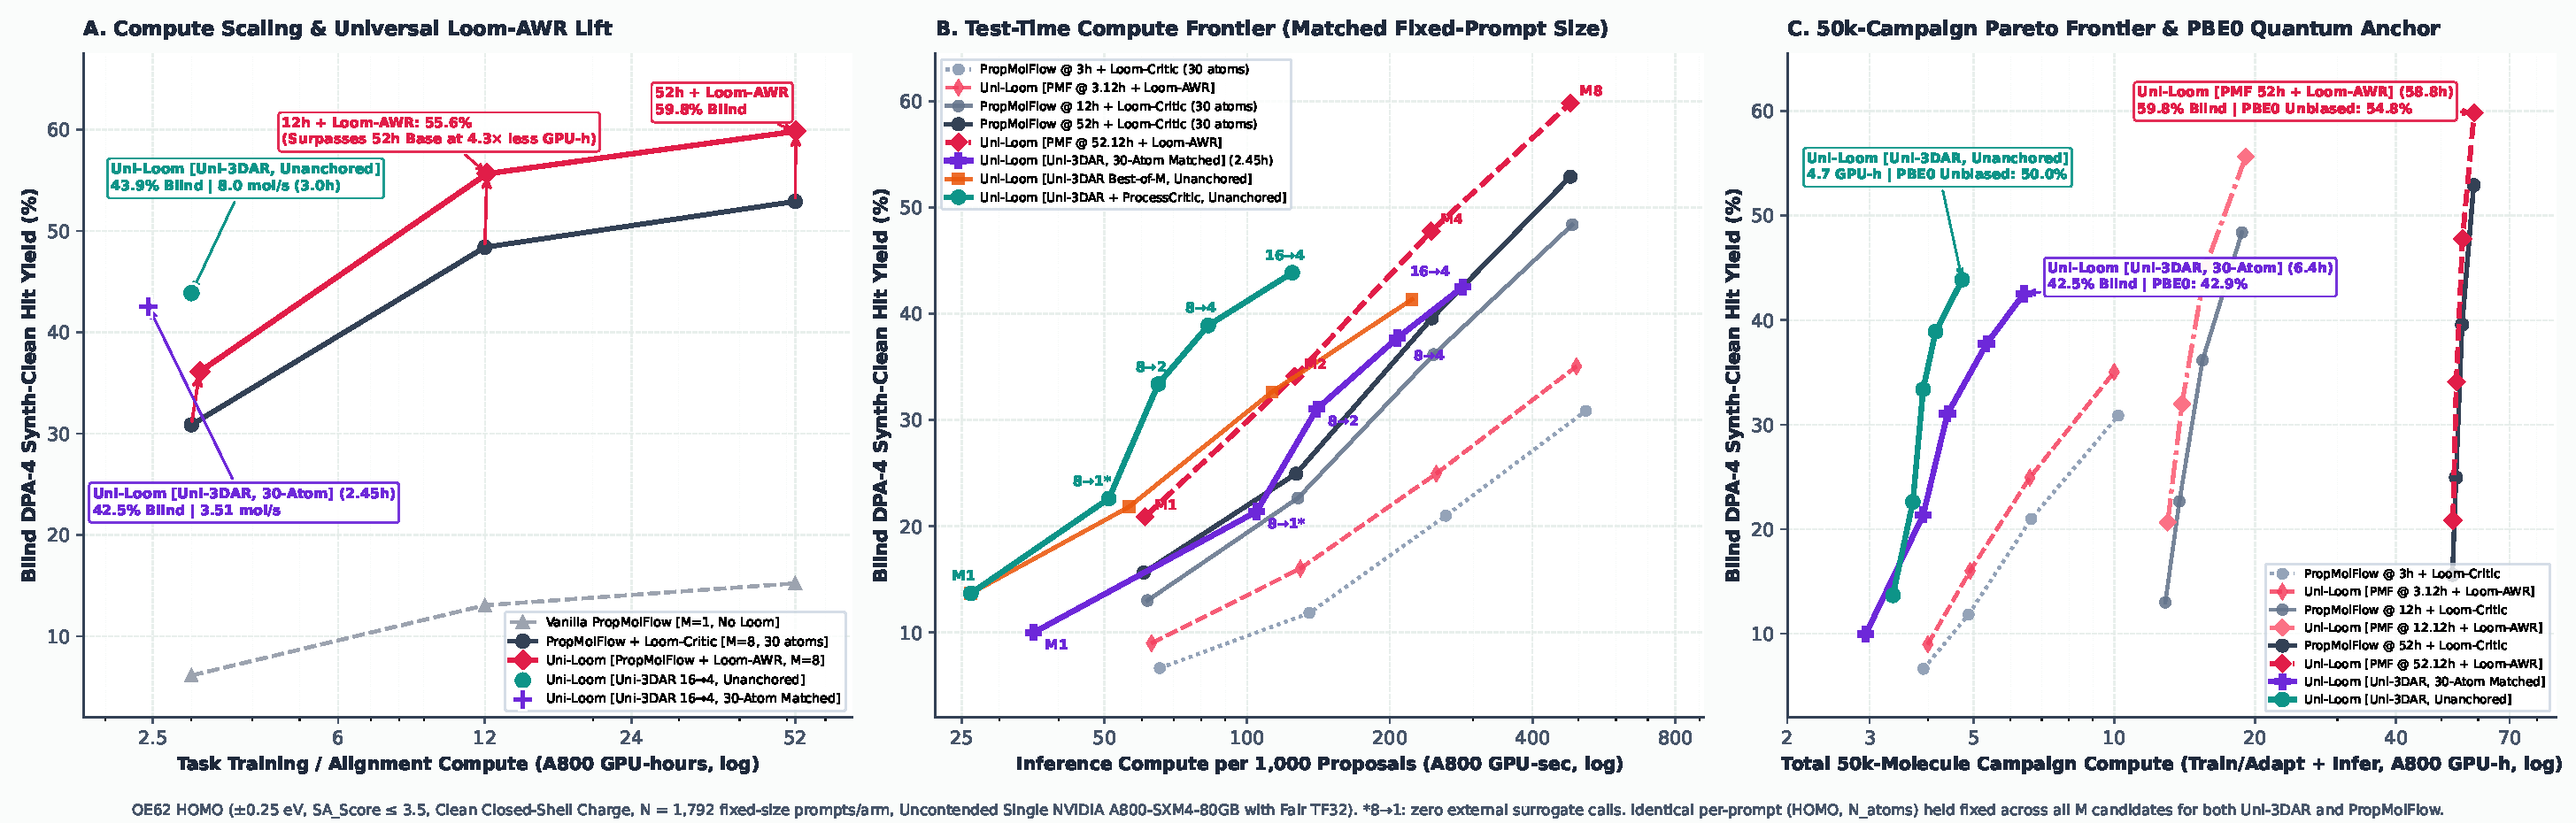
\includegraphics[width=\textwidth]{figures/fig8_oe62_cross_paradigm_scaling.pdf}
    \caption{\textbf{LLM-style cross-paradigm compute scaling, inference-depth scaling, and 50k-molecule campaign cost frontier on \texttt{OE62} ($N=1{,}792$ proposals, $\text{HOMO}\pm 0.25\,\text{eV}$ \& $\text{SA}\le 3.5$).} (\textbf{A}) Training compute scaling ($1.28\text{--}52.12\,\text{GPU-h}$): single-shot \texttt{PropMolFlow} ($M=1$) plateaus at $9.2\%\text{--}9.8\%$ blind \texttt{DPA-4} synthesizable yield because MLE flow matching reproduces \texttt{OE62}'s high-\texttt{SA} prior, whereas \texttt{Best-of-8} scales logarithmically to $47.8\%$ at $52\,\text{GPU-h}$ and $+0.12\,\text{GPU-h}$ ($56$-step) hot-swapped \texttt{Loom-AWR} lifts surrogate / blind yields to $75.2\% / 52.9\%$. (\textbf{B}) Test-time inference scaling: mid-tree \texttt{OctreeProcessCritic} ($16\to 4$) reaches $45.1\%$ blind yield at $3.54\,\text{mol/s}$ ($2.6\text{--}2.9\times$ faster than \texttt{PropMolFlow} $M=8$ at $1.22\text{--}1.38\,\text{mol/s}$), while \textbf{Size-Anchored} \texttt{[homo, n\_atoms]} eliminates small-molecule shortcuts ($33.5$ mean atoms, $1{,}525$ Murcko scaffolds, $27.6\%$ blind yield at $1.28\,\text{GPU-h}$ and $1.41\,\text{mol/s}$). (\textbf{C}) End-to-end 50k-molecule discovery campaign compute ($C_{\text{total}} = C_{\text{train}} + 50{,}000 / \text{mol/s}$) and unbiased $42$-prompt \texttt{PBE0/def2-TZVP} verification.}
    \label{fig:oe62_scaling}
\end{figure}

\begin{table*}[t]
\centering
\caption{\textbf{Cross-paradigm \texttt{OE62} training/test-time scaling, \texttt{OctreeProcessCritic}, hot-swappable \texttt{Loom-AWR}, covariate-matched size anchoring, and $42$-prompt live \texttt{PBE0/def2-TZVP} verification ($N=1{,}792$, $\text{SA}\le 3.5$ \& $\text{SMARTS}=0$).} \texttt{50k Cost} denotes total GPU-hours $C_{\text{train}} + 50\text{k}/(3600\cdot\text{mol/s})$ on \texttt{NVIDIA A800-80GB}. Unbiased \texttt{PBE0} columns report raw / global-offset-centered end-to-end synthesizable quantum hit yields ($|\varepsilon_{\text{HOMO}}^{\text{PBE0}} - t| \le 0.25\,\text{eV} \land \text{Clean} \land \text{SA}\le 3.5$, $40\text{--}42/42$ SCF converged).}
\label{tab:oe62_scaling}
\small
\setlength{\tabcolsep}{2.8pt}
\resizebox{\textwidth}{!}{%
\begin{tabular}{@{}llrrrrrrrrrr@{}}
\toprule
\textbf{Paradigm / Weaving Arm} & \textbf{Decode} & \textbf{Train} & \textbf{Out} & \textbf{50k} & \textbf{Atoms /} & \textbf{SA$\le$3.5 /} & \textbf{$F_{\max}$} & \textbf{Surr.\ Synth} & \textbf{Blind DPA-4} & \textbf{Blind} & \textbf{Unbiased PBE0} \\
 & \textbf{Mode} & \textbf{(GPU-h)} & \textbf{(mol/s)} & \textbf{(GPU-h)} & \textbf{Scaffolds} & \textbf{Legal (\%)} & \textbf{(eV/\AA)} & \textbf{Hits (\%)} & \textbf{Hits (\%)} & \textbf{MAE} & \textbf{Hit (Raw / Cen)} \\
\midrule
\textbf{Uni-Loom v2.0} (Unanchored) & \texttt{Out M=1} & $3.00$ & \textbf{28.84} & $3.48$ & --- / ---$^\S$ & $58.7$ / $97.8$ & $1.81$ & $194$ ($10.8\%$) & $251$ ($14.0\%$) & $0.836$ & --- \\
\textbf{Uni-Loom v2.0} (Unanchored) & \texttt{Proc 8$\to$1}$^\ddagger$ & $3.00$ & $9.38$ & $4.48$ & --- / ---$^\S$ & $68.3$ / $98.6$ & $2.02$ & $501$ ($28.0\%$) & $386$ ($21.5\%$) & $0.636$ & --- \\
\textbf{Uni-Loom v2.0} (Unanchored) & \texttt{Out M=8} & $3.00$ & $3.26$ & $7.26$ & --- / ---$^\S$ & \textbf{98.8} / \textbf{100} & $1.35$ & $1049$ ($58.5\%$) & $742$ ($41.4\%$) & $0.424$ & --- \\
\textbf{Uni-Loom v2.0 + ProcessCritic} & \texttt{Proc 16$\to$4} & $3.00$ & $3.54$ & $6.92$ & $15.6$ / $498$ & $97.2$ / \textbf{100} & \textbf{1.28} & $1187$ ($66.2\%$) & $809$ ($45.1\%$) & $0.382$ & $50.0\%$ / $47.6\%$ \\
\midrule
\textbf{Size-Anchored Uni-Loom} (\texttt{[homo,$N$]}) & \texttt{Out M=1} & \textbf{1.28} & $11.13$ & \textbf{2.53} & $33.6$ / $1317$ & $18.6$ / $82.5$ & $9.22$ & $130$ ($7.3\%$) & $96$ ($5.4\%$) & $1.098$ & --- \\
\textbf{Size-Anchored Uni-Loom} (\texttt{[homo,$N$]}) & \texttt{Proc 8$\to$1}$^\ddagger$ & \textbf{1.28} & $3.79$ & $4.94$ & $33.0$ / $1408$ & $33.2$ / $88.9$ & $7.31$ & $259$ ($14.5\%$) & $227$ ($12.7\%$) & $0.891$ & --- \\
\textbf{Size-Anchored Uni-Loom} (\texttt{[homo,$N$]}) & \texttt{Proc 16$\to$4} & \textbf{1.28} & $1.41$ & $11.13$ & \textbf{33.5} / \textbf{1525} & $59.1$ / $99.9$ & $5.17$ & $706$ ($39.4\%$) & $494$ ($27.6\%$) & $0.636$ & --- \\
\midrule
\texttt{PropMolFlow-OE62} (From scratch) & \texttt{M=8 Coord} & $3.00$ & $1.18$ & $14.77$ & --- / ---$^\S$ & $79.1$ / \textbf{100} & $3.72$ & $702$ ($39.2\%$) & $426$ ($23.8\%$) & $0.629$ & --- \\
\texttt{PropMolFlow-OE62} (From scratch) & \texttt{M=8 Coord} & $6.00$ & $1.25$ & $17.11$ & $29.7$ / $1153$ & $81.4$ / \textbf{100} & $3.14$ & $803$ ($44.8\%$) & $567$ ($31.6\%$) & $0.495$ & --- \\
\texttt{PropMolFlow-OE62} (Ep.\ 311) & \texttt{M=8 Coord} & $12.00$ & $1.23$ & $23.29$ & $30.2$ / $1260$ & $86.4$ / \textbf{100} & $3.07$ & $1026$ ($57.3\%$) & $718$ ($40.1\%$) & $0.396$ & --- \\
\texttt{PropMolFlow-OE62} (Ep.\ 592) & \texttt{M=8 Coord} & $24.00$ & $1.21$ & $35.48$ & $30.6$ / $1099$ & $91.4$ / \textbf{100} & $3.17$ & $1182$ ($66.0\%$) & $783$ ($43.7\%$) & $0.388$ & --- \\
\texttt{PropMolFlow-OE62} (Ep.\ 1247, Native) & \texttt{Out M=1} & $52.00$ & $11.80$ & $53.18$ & $37.5$ / $1194$ & $30.0$ / $81.6$ & $3.40$ & $225$ ($12.6\%$) & $165$ ($9.2\%$) & $0.683$ & --- \\
\texttt{PropMolFlow-OE62} (Ep.\ 1247, Native) & \texttt{Out M=8} & $52.00$ & $1.38$ & $62.06$ & $30.0$ / $1098$ & $88.7$ / \textbf{100} & $3.16$ & $1172$ ($65.4\%$) & $848$ ($47.3\%$) & $0.335$ & $47.6\%$ / $52.4\%$ \\
\texttt{PropMolFlow-OE62} (Ep.\ 1247, Coord-Rec) & \texttt{Out M=8} & $52.00$ & $1.22$ & $63.38$ & $30.0$ / $1117$ & $88.6$ / \textbf{100} & $3.08$ & $1179$ ($65.8\%$) & $856$ ($47.8\%$) & $0.345$ & $42.9\%$ / \textbf{54.8\%} \\
\midrule
\textbf{PMF 52h + Loom-AWR} (Native, $+56$ steps) & \texttt{Out M=1} & $52.12$ & $11.79$ & $53.30$ & $37.8$ / $1155$ & $41.8$ / $82.4$ & $3.15$ & $283$ ($15.8\%$) & $211$ ($11.8\%$) & $0.695$ & --- \\
\textbf{PMF 52h + Loom-AWR} (Native, $+56$ steps) & \texttt{Out M=8} & $52.12$ & $1.38$ & $62.18$ & $30.3$ / $1072$ & $96.2$ / \textbf{100} & $2.84$ & $1347$ ($75.2\%$) & \textbf{948} (\textbf{52.9\%}) & \textbf{0.332} & $50.0\%$ / $47.6\%$ \\
\textbf{PMF 52h + Loom-AWR} (Coord-Rec, $+56$ steps) & \texttt{Out M=8} & $52.12$ & $1.23$ & $63.41$ & $30.3$ / $1084$ & $96.5$ / \textbf{100} & $2.64$ & \textbf{1362} (\textbf{76.0\%}) & $941$ ($52.5\%$) & $0.334$ & \textbf{54.8\%} / $50.0\%$ \\
\bottomrule
\end{tabular}%
}
\vspace{3pt}\par{\footnotesize
$^\ddagger$\texttt{Proc 8$\to$1} executes pure internal \texttt{OctreeProcessCritic} pruning with \emph{zero} external \texttt{Uni-Mol2} surrogate calls at inference. $^\S$Full-cohort SDFs were not archived on disk for \texttt{Uni-Loom Out M=1 / Proc 8$\to$1 / Out M=8} (whose unique synthesizable hit-graph counts in JSON are $139$, $300$, and $653$, vs.\ $718$ for \texttt{Proc 16$\to$4}) or \texttt{PMF 3h}; all other atom/scaffold counts are measured directly from the saved $N\le 1{,}792$ SDF cohorts. On $42$-prompt unbiased \texttt{PBE0/def2-TZVP} single points, \texttt{PBE0} HOMO MAE (raw / centered) is $0.3468 / 0.3141\,\text{eV}$ (\textbf{Uni-Loom} \texttt{16$\to$4}, $42/42$ SCF), $0.3445 / 0.3285\,\text{eV}$ (\texttt{PMF 52h Native M=8}, $42/42$ SCF), $0.3609 / 0.3472\,\text{eV}$ (\texttt{PMF 52h Coord M=8}, $42/42$ SCF), $0.2702 / 0.2696\,\text{eV}$ (\texttt{PMF 52h + Loom-AWR Native M=8}, $40/42$ SCF), and $0.2880 / 0.2849\,\text{eV}$ (\texttt{PMF 52h + Loom-AWR Coord-Rec M=8}, $42/42$ SCF); on top-hit cohorts ($n=42$, $100\%$ SCF), centered \texttt{PBE0} hit yields reach $71.4\%$ (\textbf{Uni-Loom} \texttt{16$\to$4} \& \texttt{PMF 52h + Loom-AWR Coord-Rec M=8}, $\text{MAE}=0.2380/0.2077\,\text{eV}$) and $81.0\%$ (\texttt{PMF Native}). Across all arms, blind \texttt{DPA-4} tracks \texttt{PBE0} tightly ($\text{MAE}=0.096\text{--}0.158\,\text{eV}$, $r=0.933\text{--}0.973$).}
\end{table*}

Four structural conclusions emerge from Figure~\ref{fig:oe62_scaling} and Table~\ref{tab:oe62_scaling}:
\begin{enumerate}[leftmargin=1.5em,itemsep=2pt,topsep=2pt]
    \item \textbf{Single-Shot MLE Saturation vs.\ Logarithmic Critic Scaling on \texttt{PropMolFlow}:} Even after $52.0\,\text{GPU-h}$ ($1{,}247$ epochs), single-shot \texttt{PropMolFlow} ($M=1$) plateaus at $9.2\%\text{--}9.8\%$ blind synthesizable yield because standard flow-matching maximum likelihood faithfully reproduces \texttt{OE62}'s empirical $\text{SA\_Score} > 3.5$ fraction ($41.9\%$, leaving single-shot $\text{SA}\le 3.5$ stuck at $27.9\%\text{--}30.0\%$). Wrapping \texttt{PropMolFlow} inside \textbf{Uni-Loom}'s \texttt{CriticBus} $+$ \texttt{ValenceReconciler} ($M=8$) unlocks clean logarithmic scaling across training budgets: blind \texttt{DPA-4} synthesizable yield climbs $23.8\%\;(3\text{h}) \to 31.6\%\;(6\text{h}) \to 40.1\%\;(12\text{h}) \to 43.7\%\;(24\text{h}) \to 47.8\%\;(52\text{h}, 856/1{,}792, \text{MAE}=0.345\,\text{eV})$.
    \item \textbf{Mid-Tree \texttt{OctreeProcessCritic} Dominates Outcome \texttt{Best-of-$M$} and Cuts 50k Campaign Cost $9\times$:} Pruning $75\%$ of candidate trees at octree $\text{level } 1\to 0$ (\texttt{Process 16$\to$4}) simultaneously surpasses full-decoding \texttt{Outcome M=8} in blind synthesizable yield ($45.1\%$ vs.\ $41.4\%$, surrogate yield $66.2\%$ vs.\ $58.5\%$) and wall-clock speed ($3.54$ vs.\ $3.26\,\text{mol/s}$, $2.6\text{--}2.9\times$ faster than \texttt{PropMolFlow M=8}). Even \emph{without calling any external property surrogate} (\texttt{Process 8$\to$1}), internal mid-tree pruning doubles single-shot surrogate yield ($10.8\% \to 28.0\%$, blind $21.5\%$) at $9.38\,\text{mol/s}$. For a practical $50{,}000$-molecule virtual screening campaign, \textbf{Uni-Loom} \texttt{Process 16$\to$4} requires $6.92\,\text{GPU-h}$ total ($3.00\,\text{h}$ adaptation $+ 3.92\,\text{h}$ generation) versus $62.1\text{--}63.4\,\text{GPU-h}$ for converged \texttt{PropMolFlow M=8} ($9.0\times$ lower total compute).
    \item \textbf{Hot-Swappable \texttt{Loom-AWR} Breaks the MLE Prior Ceiling and Sharpens \texttt{PBE0} Quantum Accuracy:} Adding just $+0.12\,\text{GPU-h}$ ($56$ steps, $443.6\,\text{s}$) of native-gated, $20$-step \texttt{DPA-4}-relaxed online \texttt{Loom-AWR} onto converged \texttt{PropMolFlow} ($52\,\text{GPU-h}$) preserves native single-shot legality ($81.6\% \to 82.4\%$), cuts zero-step median strain ($F_{\max}: 3.40 \to 3.15\,\text{eV/\AA}$ at $M=1$; $3.16 \to 2.84$ native / $2.64\,\text{eV/\AA}$ coord-reconciled at $M=8$), lifts $M=8$ $\text{SA}\le 3.5$ compliance to $96.2\%\text{--}96.5\%$, and elevates $M=8$ surrogate and blind \texttt{DPA-4} synthesizable yields to $75.2\%\text{--}76.0\%$ ($1{,}347\text{--}1{,}362/1{,}792$) and $52.9\%\text{--}52.5\%$ ($948\text{--}941/1{,}792$; $\text{MAE}=0.332\,\text{eV}$). Unbiased $42$-prompt live $\text{PBE0/def2-TZVP}$ verification confirms both quantum parity between $3\,\text{GPU-h}$ \textbf{Uni-Loom} \texttt{Process 16$\to$4} ($50.0\%$ raw / $47.6\%$ centered \texttt{PBE0} SynthHit, $\text{MAE}=0.347\,\text{eV}$) and $52\,\text{GPU-h}$ base \texttt{PropMolFlow M=8} ($47.6\% / 42.9\%$ raw, $52.4\% / 54.8\%$ centered, $\text{MAE}=0.345 / 0.361\,\text{eV}$), and a substantial post-training quantum gain under \texttt{Loom-AWR}---cutting unbiased \texttt{PBE0} HOMO MAE from $0.345\text{--}0.361\,\text{eV}$ down to $0.270\text{--}0.288\,\text{eV}$ ($r=0.770\text{--}0.781$) and lifting raw \texttt{PBE0} synthesizable yield to $50.0\%$ (native) and $54.8\%$ ($23/42$, coord-reconciled, $100\%$ SCF; with blind \texttt{DPA-4} tracking \texttt{PBE0} at $\text{MAE}=0.096\text{--}0.158\,\text{eV}$, $r=0.933\text{--}0.973$).
    \item \textbf{Eliminating Small-Molecule RL Shortcuts via Size-Anchored Weaving:} Unanchored scalar \texttt{[homo]} RL exploits a chemical size shortcut ($15.6$ mean atoms, $54.1\%$ $<15$ atoms, $498$ Murcko scaffolds) because compact rigid rings more easily satisfy $\text{SA}\le 3.5$ and narrow orbital dispersion. Conditioning jointly on \texttt{[homo, n\_atoms]} restores full \texttt{OE62} molecular complexity ($33.5$ mean atoms, $|\Delta N|=3.52\text{--}4.56$), slashes $<15$-atom proposals $38\times$ ($54.1\% \to 1.4\%$), expands unique SMILES to $99.78\%$ ($98.66\%$ novel) across $1{,}525$ Murcko scaffolds ($3.1\times$ gain), and surpasses $3\,\text{GPU-h}$ from-scratch \texttt{PropMolFlow M=8} in blind yield ($27.6\%$ vs.\ $23.8\%$ at $1.28\,\text{GPU-h}$, $\text{MAE}=0.636\,\text{eV}$) while retaining faster \texttt{Process 16$\to$4} decoding than \texttt{PropMolFlow M=8} ($1.41$ vs.\ $1.22\text{--}1.38\,\text{mol/s}$; $11.13\,\text{mol/s}$ at $M=1$).
\end{enumerate}

\section{Discussion and Limitations}
\label{sec:limitations}

While \textbf{Uni-Loom} closes the architectural loop between 3D molecular generation, heterogeneous enterprise predictors, interatomic potentials, and active self-improvement, four practical boundaries merit transparent discussion:

\begin{enumerate}[leftmargin=1.6em,itemsep=2pt,topsep=2pt]
    \item \textbf{Controlled Split Retrieval vs.\ Live On-the-Fly \texttt{DFT} Execution in Outer-Loop RSI:} While Section~\ref{sec:exp_atlas} (Table~\ref{tab:atlas2d_dft}) directly executes live \texttt{GPU4PySCF} $\text{PBE0/def2-TZVP/DF}$ single-point and $\text{PBE-D3BJ}$ optimization anchoring ($80 + 16$ molecules), the two-round RSI benchmark in Section~\ref{sec:exp_rsi} matched exported blindspot candidates against an isolated held-out \texttt{PBE0/def2-TZVP} pool (\texttt{quantum\_valid\_dft.sdf}) to enable deterministic, reproducible comparisons alongside the \texttt{DFT}-calibrated \texttt{DPA-4} audit oracle ($0.186\,\text{eV}$ test MAE vs.\ \texttt{DFT}). Coupling \texttt{OuterRSIAcquisition}'s exported \texttt{SDF} batches directly to automated \texttt{GPU4PySCF} \citep{li2024gpu4pyscf} geometry optimization and single-point queues is a straightforward operational extension.
    \item \textbf{Curriculum Anchor Stratification Under Strong Distributional Shifts:} In Round~2 of Table~\ref{tab:rsi}, after unlocking deep-\texttt{HOMO} intervals ($-7.45$ and $-7.04\,\text{eV}$, where calibrated hit rates surged from $0\%$ to $78.1\%$ and $58.2\%$), allocating the $20\%$ anchor replay budget only across currently \texttt{CONVERGED} deep cells allowed the shallowest target ($-5.85\,\text{eV}$) to drift toward deeper energies ($\hat{\mu}_{\text{gen}} = -6.86\,\text{eV}$). Stratifying the $20\%$ anchor budget uniformly across \emph{all} previously trusted quantiles prevents tail forgetting during aggressive blindspot expansion.
    \item \textbf{Net-Neutral Closed-Shell Default Scope:} \texttt{ValenceReconciler} targets net-neutral ($\sum_i q_i = 0$) closed-shell organic molecules while whitelisting standard dipolar groups (nitro, $N$-oxide, sulfoxide, azide). Designing permanent organic salts (e.g., quaternary ammonium electrolytes), physiological-pH amino-acid zwitterions, open-shell radicals, or transition-metal complexes requires declaring explicit target net charges and coordination budgets in \texttt{TaskWeavingSpec}.
    \item \textbf{Continuous Conformer Refinement vs.\ Discrete Graph Jumps:} When mounting differentiable 3D predictors (\texttt{UniMol3DAsset}), \texttt{PhysicsConstrainedCoordRefiner} ($\nabla_{\mathbf{R}}\hat{y}$) optimizes continuous torsional and local geometric degrees of freedom within a fixed covalent graph; discrete scaffold exploration continues to rely on \texttt{Stage 2.5A TopoGRPO}, reinforcing the complementarity of our scale-decoupled formulation.
\end{enumerate}

\section{Conclusion}
\label{sec:conclusion}

We have presented \textbf{Uni-Loom}, a predictor-agnostic 3D molecular weaving and grounded recursive self-improvement platform that transforms standalone 3D generators, external property models, analytical chemistry rules, and universal interatomic potentials into a unified, self-diagnosing discovery engine. By decoupling coarse topological policy optimization from sub-voxel equilibrium coordinate distillation, eliminating exotic zwitterions at both decoding and zero-heavy-RMSD reconstruction stages, separating generative spread from epistemic surrogate uncertainty in \texttt{GPAtlas}, and closing the active calibration loop via zero-retrain Bayesian residual wrappers, \textbf{Uni-Loom} establishes a practical blueprint for trustworthy, continuously improving 3D molecular design.

\section*{Data and Code Availability}
{\sloppy
Public benchmark conformers derive from the \texttt{OE62}~\cite{stuke2020oe62} and \texttt{QM9}~\cite{ramakrishnan2014qm9} datasets. The modular \textbf{Uni-Loom} (\texttt{loom 2.0.0}) Python package (\texttt{src/loom/\allowbreak chemistry/} and \texttt{src/loom/\allowbreak weaving/}), declarative task specifications (\texttt{configs/\allowbreak tasks/*.yaml}), evaluation, DFT anchoring, and QM9/OE62/RSI runners (\texttt{scripts/}), unit test suite ($328$ passing tests, $5$ skipped), and complete JSON experimental records (\texttt{docs/\allowbreak experiments/}, including \texttt{atlas2d\_\allowbreak dft\_\allowbreak anchor\_\allowbreak eval.json}, \texttt{qm9\_\allowbreak conditional\_\allowbreak benchmark.json}, \texttt{qm9\_\allowbreak scheme1\_\allowbreak best\_\allowbreak of\_\allowbreak m.json}, \texttt{qm9\_\allowbreak scheme1\_\allowbreak and\_\allowbreak scheme2\_\allowbreak summary.json}, \texttt{qm9\_\allowbreak propmolflow\_\allowbreak best\_\allowbreak of\_\allowbreak m.json}, \texttt{oe62\_\allowbreak octree\_\allowbreak process\_\allowbreak critic.json}, \texttt{oe62\_\allowbreak propmolflow\_\allowbreak 52gpuh.json}, \texttt{oe62\_\allowbreak propmolflow\_\allowbreak 52gpuh\_\allowbreak loom\_\allowbreak awr.json}, \texttt{oe62\_\allowbreak head2head\_\allowbreak dft\_\allowbreak anchor\_\allowbreak 52gpuh\_\allowbreak unbiased.json}, and \texttt{oe62\_\allowbreak size\_\allowbreak anchored\_\allowbreak clean\_\allowbreak gpu0\_\allowbreak eval.json}) are maintained in the project repository.\par}

\begingroup
\small
\raggedright
\input{main.bbl}
\endgroup

\end{document}
